\documentclass{scrartcl} %instead of article to allow for use of subtitle
\setkomafont{disposition}{\normalfont\bfseries} %need this for scrartcl for title font to look normal
\usepackage{geometry} 
\geometry{letterpaper} 
%%%% Uncomment below to begin paragraphs with an empty line %%%%
\usepackage[parfill]{parskip} 
\usepackage{graphicx}
\usepackage{amssymb}
\usepackage{moreverb}
%\usepackage[section]{placeins}
%\usepackage[below]{placeins}
\usepackage{epstopdf}

% Begin from doxygen


%\usepackage{makeidx}
%\usepackage{natbib}
\usepackage{graphicx}
\usepackage{multicol}
\usepackage{float}
\usepackage{listings}
\usepackage{color}
%\usepackage{ifthen}
\usepackage[table]{xcolor}
\usepackage{textcomp}
\usepackage{alltt}
\usepackage[pdftex,
            pagebackref=true,
            colorlinks=true,
            linkcolor=blue,
            urlcolor=blue,
            unicode
           ]{hyperref}
%\usepackage[utf8]{inputenc}
%\usepackage{mathptmx}
%\usepackage[scaled=.90]{helvet}
%\usepackage{courier}
%\usepackage{sectsty}
\usepackage[titles]{tocloft}
\usepackage{doxygen}
\lstset{language=C++,inputencoding=utf8,basicstyle=\footnotesize,breaklines=true,breakatwhitespace=true,tabsize=8,numbers=left }
%\makeindex
\setcounter{tocdepth}{3}
%\renewcommand{\footrulewidth}{0.4pt}
%\renewcommand{\familydefault}{\sfdefault}
%\hfuzz=15pt
%\setlength{\emergencystretch}{15pt}
%\hbadness=750
%\tolerance=750

% End from doxygen

%\DeclareGraphicsRule{.tif}{png}{.png}{`convert #1 `dirname #1`/`basename #1 .tif`.png}
\newcommand\bslash{\char`\\}
\newcommand\lt{\char`\<}
\newcommand\gt{\char`\>}
\newcommand{\tab}{\hspace*{2em}}
\newcommand{\supers}[1]{\ensuremath{^\textrm{{\scriptsize #1}}}}
\newcommand{\subs}[1]{\ensuremath{_\textrm{{\scriptsize #1}}}}
\newcommand{\notebox}[1]{ \begin{center}\framebox[5.5in]{\begin{minipage}[t]{5.0in}\textbf{Note: }#1\end{minipage}}\end{center}}

\title{SSC Reference Manual
\subtitle{SDK 2017.1.17 Revision 2, SSC 172}}
\author{Aron Dobos and Paul Gilman}

\begin{document}

\maketitle
\vspace{2.5in}
\begin{abstract}
The SSC (SAM Simulation Core) software library is the collection of simulation modules used by the National Renewable Energy Laboratory's  System Advisor Model (SAM).  The SSC application programming interface (API) allows software developers to integrate SAM's modules into web and desktop applications. The API includes mechanisms to set input variable values, run simulations, and retrieve values of output variables. The SSC modules are available in pre-compiled binary dynamic libraries minimum system library dependencies for Windows, OS X, and Linux operating systems. The native API language is ISO-standard C, and language wrappers are available for C\#, Java, MATLAB, Python, and PHP. The API and model implementations are thread-safe and reentrant, allowing the software to be used in a parallel computing environment.

This document describes the SSC software architecture, modules and data types, provides code samples, introduces SDKtool, and describes the language wrappers.
\end{abstract} 

\newpage
\tableofcontents
%%\listoffigures
%%\listoftables
\newpage

\section{Overview}
\label{sec_overview}

The SAM simulation core (SSC) software development kit (SDK) provides tools for creating models of renewable energy systems using the SSC library. The System Advisor Model (SAM) desktop application is a user-friendly front-end for the SSC library that uses SSC modules to perform all system performance and financial calculations. This manual assumes that the reader is familiar with SAM's suite of performance and financial models, input and output variables, and other capabilities. The SDK consists of the application programming interface (API), library, programming language wrappers, integrated development environment, code samples, and this manual.

\subsection{Framework Description}

The SSC framework provides a generic mechanism for running modules, setting values of module inputs, and reading values of module outputs. The mechanisms are generic because they do not depend on the module. For example, the same mechanism provides access to the PVWatts (\texttt{pvwattsv5}) and Utility Single Owner (\texttt{singleowner}) modules.  

Using an SSC module is analogous to calling a function in a programming language: you pass parameter values to the function, run the function, and then read values returned by the function.  In SSC, you store input variables in a data container, run the module, and retrieve outputs from the same data container:

\begin{enumerate}
\item Create a data container of type \texttt{ssc\_data\_t} for model input variables.
\item Call a simulation module such as \texttt{pvwattsv5} or \texttt{singleowner}, both of type \texttt{ssc\_module\_t} to process variables in the data container. If the module runs successfully, it populates the data container with output variables. If it fails, it generates error messages.
\item Retrieve results from the data container.
\end{enumerate}

\subsection{Modeling an Energy System}
\label{sec_modeling_systems}

The SSC simulation modules process weather data files, simulate the performance of energy systems and their components, and calculate financial cash flows and metrics.

Creating a model of a renewable energy system in SSC involves running a set of modules to represent the physical system and a financing structure. For example, a model of a residential photovoltaic system might require four modules:

\begin{itemize}
\item \texttt{pvwattsv5}: Defines the system's design parameters and calculates the hourly output over a single year.
\item \texttt{utilityrate}: Calculates the value of energy generated by the system for each hour of the first year, and as an annual total for subsequent years.
\item \texttt{cashloan}: Calculates financial metrics including the cost of energy, net present value, based on installation and operating costs, incentives, taxes, and loan parameters.
\end{itemize}

The following pseudocode shows what a program that calculates the net present value of a residential photovoltaic system would look like. It calls the modules in the order shown above, with some outputs of each module serving as inputs for the next.

\begin{enumerate}
\item Create data container
\item Assign values to pvwattsv5 input variables
\item Run pvwattsv5
\item Retrieve system hourly output from data container
\item Assign values to utilityrate input variables
\item Run utilityratev3
\item Retrieve energy values from data container
\item Assign values to cashloan input variables
\item Run cashloan
\item Retrieve net present value from data container
\item Display net present value
\end{enumerate}

\section{An Example: Running PVWatts}
\label{sec_pvwatts_example}

In this section, we write a short command-line C program to calculate the total annual energy production of a 1 kW PV system at a particular location. The program performs the following tasks:

\begin{enumerate}
\item Create Data Container
\item Assign values to the \texttt{pvwattsv1} input variables
\item Run \texttt{pvwattsv5}
\item Display the total annual output
\end{enumerate}

The complete source code for this program is included with the SSC SDK in the file \texttt{example1\_pvwatts.c}.

This example is written in C, SSC's native language. The language interfaces included with the SDK and described in \S\ref{sec_language_interfaces} allow you to use SSC in programs written in other languages.

You can also use the scripting language included with SDKtool to run SSC modules and build models based on SSC as described in \S\ref{sec_sdktool}.

\notebox{The desktop version of SAM can export input data from a SAM project file to a ready-to-run C program. See the \emph{Software Development Kit} topic in SAM's Help system for details.}

\subsection{Write the program skeleton}

To start, we'll write the program skeleton. It includes the standard input-output and  \texttt{sscapi.h} header files. The SSC API header file must be included in any program that uses SSC functions.

The main function gives the weather file as a command line argument. It must be in one of the formats that \texttt{pvwattsv5} can read: SAM CSV, TMY2, TMY3, or EPW.

\begin{verbatimtab}[4]
#include <stdio.h>
#include "sscapi.h"

int main(int argc, char *argv[])
{
	if ( argc < 2 )
	{
		printf("usage: pvwatts.exe <weather-file>\n");
		return -1;
	}
 
	// run PVWatts simulation for the specified weather file
	
	return 0;
}
\end{verbatimtab}

\subsection{Create the data container}

Next we replace the comment in the program skeleton with code that creates the SSC data container that will store all input and output variables.
 
The \texttt{ssc\_data\_create()} function returns a value of type \texttt{ssc\_data\_t}, which we assign to the variable \texttt{data}.

If the function call fails due to the system having run out of memory, the function returns \texttt{NULL}. By checking the function's return value, we can be sure that it succeeded in creating the data container.

\begin{verbatimtab}[4]
	ssc_data_t data = ssc_data_create();
	if ( data == NULL )
	{
		printf("error: out of memory.\n");
		return -1;
	}
\end{verbatimtab}

\subsection{Assign values to the module input variables}

The \texttt{pvwattsv1} module requires six input variables. You can use the approach described in \S\ref{sec_variable_docs} to list information about a module's input and output variables. You can also use the SDKtool module browser described in \S\ref{sec_sdktool} to explore the variables.

The \texttt{pvwattsv1} input variables are numbers, except for the weather file name which is a string. SSC also supports array, matrix, and table data types.

\begin{verbatimtab}[4]
	ssc_data_set_string( data, "solar_resource_file", argv[1] ); // weather file name
	ssc_data_set_number( data, "system_capacity", 1.0f );  // 1 kW DC system
	ssc_data_set_number( data, "losses", 14.0f );      // system losses, in \%
	ssc_data_set_number( data, "array_type", 0 );      // fixed tilt system
	ssc_data_set_number( data, "tilt", 20 );           // 20 degree tilt
	ssc_data_set_number( data, "azimuth", 180 );       // south facing
	ssc_data_set_number( data, "adjust:constant", 0.0f ); // energy adjustment, 0 \% losses
\end{verbatimtab}

\subsection{Run the module}
\label{sec_run_module}

To run the \texttt{pvwattsv1} module, we first create an instance of the module by passing its name as a string to the \texttt{ssc\_module\_create()} function, and then run the module. 

The \texttt{ssc\_module\_create()} function may return \texttt{NULL} if it does not recognize the name or if the system is out of memory.

\begin{verbatimtab}[4]
	ssc_module_t module = ssc_module_create( "pvwattsv5" );
	if ( NULL == module )
	{
		printf("error: could not create 'pvwattsv5' module.\n");
		ssc_data_free( data );
		return -1;
	}
\end{verbatimtab}

The \texttt{ssc\_module\_exec} runs the module we created with the data container stored in \texttt{data} and returns a value of 1 if the simulation succeeds. If any of the module's required input variables use the wrong data type or a value that does not meet constraints, or if the simulation fails for some other reason, it returns a value of 0.

\begin{verbatimtab}[4]
	if ( ssc_module_exec( module, data ) == 0 )
	{
		printf("error during simulation.\n");
		ssc_module_free( module );
		ssc_data_free( data );
		return -1;
	}
\end{verbatimtab}

The \texttt{ssc\_module\_exec()} function is one way to run a module. For more details about the function and others that run modules with different options for handling errors, see \S\ref{sec_errors}.

\subsection{Retrieve results from the data container and display them}

If the simulation succeeds, we can retrieve the model outputs that we want from the data container. For this example, the only output we need is the hourly AC energy produced by the system, which we will use to calculate the system's total annual AC energy in kWh. For the \texttt{pvwattsv1} module, the system's hourly energy is stored in the \texttt{ac} variable in Wh.

\begin{verbatimtab}[4]
	double ac_total = 0;
	int len = 0;
	ssc_number_t *ac = ssc_data_get_array( data, "ac", &len );
	if ( ac != NULL )
	{
		int i;
		for ( i=0; i<len; i++ )
			ac_total += ac[i];
		printf("ac: %lg kWh\n", ac_total*0.001 );
	}
	else
	{
		printf("variable 'ac' not found.\n");
	}
\end{verbatimtab}

\subsection{Cleaning up}

Now that we're done with the simulation, we should free the memory associated with the module and data container. The \texttt{ssc\_module\_free()} function releases the module, and \texttt{ssc\_data\_free()} frees memory associated with the data container. 

\begin{verbatimtab}	
	ssc_module_free( module );
	ssc_data_free( data );
\end{verbatimtab}

\subsection{Compile and run the C program}

This description explains how to compile and run the C program in Windows using the  MinGW development environment, assuming we saved the code to the file \texttt{example1\_pvwatts.c}. This example was tested with MinGW gcc version 4.6.2.

To compile and run the program, the following files must be in the same folder:

\begin{itemize}
\item The \texttt{.c} file containing the program code
\item The \texttt{sscapi.h} header file
\item The dynamic library file \texttt{ssc.dll}
\item The \texttt{daggett.tm2} weather file
\end{itemize}

To compile the program, type the following command at the Windows command prompt:

\begin{verbatim}
c:\> gcc example1_pvwatts.c ssc.dll -o pvwatts.exe
\end{verbatim}

To run the program, specify a weather file on the command line. Here, we use the TMY2 file for Daggett, California:

\begin{verbatim}
c:\> pvwatts.exe daggett.tm2
ac: 1808.87 kWh
\end{verbatim}

\subsection{Some additional comments}

The \texttt{ssc\_data\_t} and \texttt{ssc\_module\_t} data types are opaque references to internally defined data structures.  The only proper way to interact with variables of these types is using the defined SSC function calls.  As listed in the \texttt{sscapi.h} header file, both are typedef'd as \texttt{void*}.


\section{Data Variables}
\label{sec_variables}

Simulation model inputs and outputs are stored in a data container of type \texttt{ssc\_data\_t}, which is simply a collection of named variables.  Internally, the data structure is an unordered map (hash table), permitting very fast lookup of variables by name.  Every input and output variable in SSC is designated a \emph{name}, a \emph{variable type}, and a \emph{data type}, along with other meta data (labels, units, etc). 

\subsection{Variable Names}

The variable name is how SSC identifies data, and your program must use the predefined names to refer to the variables. A variable names may contain letters, numbers, and underscores. SSC does not distinguish between uppercase and lowercase letters, so \texttt{Beam\_Irradiance} is the same variable as \texttt{beam\_irradiance}.

\subsection{Variable Types}

The \emph{variable type} identifies each variable as an input, output, or in-out variable.  In the SSC API, these values are defined by the following constants listed below.

\begin{verbatimtab}
#define SSC_INPUT 1
#define SSC_OUTPUT 2
#define SSC_INOUT 3
\end{verbatimtab}

Input variables must be defined before calling a module. Output variables are calculated by the module, which adds them to the data container after running. In-out variables must be defined before running the module, which changes its value after running.

From the perspective of the data container, inputs and outputs are equivalent. The data container is just a pile of data, and provides no information about whether its variables are input, output, or in-out variables. Only is only the simulation modules specify the variable type.

\subsection{Data Types}

Every variable in SSC is assigned a particular data type. Each simulation module specifies the data type of each variable it requires as input and output.

SSC can work with numbers, text strings, one-dimensional arrays, two-dimensional matrices, and tables. The data type constants are listed below.

\begin{verbatimtab}
#define SSC_INVALID 0
#define SSC_STRING 1
#define SSC_NUMBER 2
#define SSC_ARRAY 3
#define SSC_MATRIX 4
#define SSC_TABLE 5
\end{verbatimtab}

All numbers are stored using the \texttt{ssc\_number\_t} data type.  By default, this is a typedef of the 32-bit floating point C data type (\texttt{float}).  The purpose of using \texttt{float} instead of the 64-bit \texttt{double} is to save memory.  While a simulation module may perform all of its calculations internally using 64-bit precision floating point, the inputs and results are transferred into and out of SSC using the smaller data type.

Arrays (1-D) and matrices (2-D) store numbers only. There is no provision for arrays or matrices of text strings, or arrays of tables.  Arrays and matrices are optimized for efficient storage and transfer of large amounts of numerical data.  For example, a photovoltaic system simulation at 1 second timesteps for a whole year would produce 525,600 data points, and potentially several such data vectors might be reported by a single simulation model.  This fact underscores the reasoning behind our decision to use the 32-bit floating point data type: just 20 vectors of 525,600 values each would require 42 megabytes of computer memory.

SSC stores all numbers are stored as floating point. A module may limit a numeric variable to an integer, boolean (0 or 1), or positive value using a constraint flag as described in \S\ref{sec_def_const}. The constraints are checked automatically before the module runs.

Text strings (\texttt{SSC\_STRING})  are stored as 8-bit characters.  SSC does not support multi-byte or wide-character string representations, and all variable names and labels use only the 7-bit ASCII Latin alphabet.  Consequently, text is stored as null ('\textbackslash 0') terminated \texttt{char*} C strings.  The weather file name is a common input variable that uses the \texttt{SSC\_STRING} data type.

The table (\texttt{SSC\_TABLE}) data type is the only hierarchical data type in SSC.  It allows a simulation module to receive or return outputs in a structured format with named fields.  A table is a named variable that is itself a data container, which can store any number of named variables of any SSC data type.  Currently, most SSC modules do not make heavy use of tables, but they are fully implemented and supported for future modules that may require them.

\subsection{Variable Documentation}
\label{sec_variable_docs}

Each module defines all of the input variables it requires and output variables it produces. The SSC functions described below return information about the variables defined by a module. Each variable specifies the information shown in Table~\ref{tab_varinfo}.

\begin{table}[ht]
\begin{center}
\begin{tabular}{ll}
Field & Description\\
\hline
Variable type & \texttt{SSC\_INPUT}, \texttt{SSC\_OUTPUT}, \texttt{SSC\_INOUT} \\
Data type & \texttt{SSC\_NUMBER}, \texttt{SSC\_STRING}, \texttt{SSC\_ARRAY}, \texttt{SSC\_MATRIX}, \texttt{SSC\_TABLE} \\
Name & Variable name (case insensitive) \\
Label & A description of the variable's purpose \\
Units & The units of the numerical value(s) \\
Meta & Additional information. Could specify encoding of values, see below. \\
Group & General category of variable, e.g. "Weather'', "System Input'' \\
Required & Specifies whether the variable must be assigned a value. See \S\ref{sec_def_const} \\
Constraints & Constraints on the values or number of values. See \S\ref{sec_def_const} \\
UI Hints & Suggestions on how to display this variable.  Currently unused. \\
\end{tabular}
\caption{Variable information provided by SSC}
\label{tab_varinfo}
\end{center}
\end{table}

The \texttt{ssc\_module\_var\_info()} function queries a module and returns a \texttt{ssc\_info\_t} reference. The \texttt{while} loop below calls \texttt{ssc\_module\_var\_info()} until all of the module's variables have been displayed. This example assumes that the variable \texttt{module} was successfully created as described in \S\ref{sec_explicit_modules} or in the example in \S\ref{sec_run_module}. You can use a similar approach to list available modules with their descriptions as described in \S\ref{sec_modules_querying}.

\begin{verbatimtab}[4]
int i=0;
ssc_info_t p_inf = NULL;
while ( p_inf = ssc_module_var_info( module, i++ ) )
{
	// var_type: SSC_INPUT, SSC_OUTPUT, SSC_INOUT
	int var_type = ssc_info_var_type( p_inf );

	// data_type: SSC_STRING, SSC_NUMBER, SSC_ARRAY, SSC_MATRIX, SSC_TABLE   
	int data_type = ssc_info_data_type( p_inf );
      
	const char *name = ssc_info_name( p_inf );
	const char *label = ssc_info_label( p_inf );
	const char *units = ssc_info_units( p_inf );
	const char *meta = ssc_info_meta( p_inf );
	const char *group = ssc_info_group( p_inf );
	const char *required = ssc_info_required( p_inf );
	const char *constraints = ssc_info_constrants( p_inf );

	// here, you can print all of this data to text file
	// or present it in another way to the user

	printf( "%s %s (%s) %s\n", name, label, units, meta );
}

\end{verbatimtab}

Another option for exploring a module's variables is SDKtool. It displays the variables in an interactive GUI spreadsheet-style interface described in \S\ref{sec_module_browser}.

\subsection{Required Variables, Constraints, and Default Values}
\label{sec_def_const}

The \emph{Required} and \emph{Constraints} fields of a variable's documentation indicate whether the variable is required or optional, and whether it has a default value. Table \ref{tab_required} shows the \emph{Required} flags and their meanings, and Table \ref{tab_constraints} shows the \emph{Constraints} flags. 

\begin{table}[ht]
\begin{center}
\begin{tabular}{p{0.75in}p{4.75in}}
Flag & Description\\
\hline
\texttt{*} &  Variable requires a user-specified value. If a required variable is not assigned a value before running the module, the simulation fails.\\
\texttt{?} & Optional variable. SSC ignores the variable unless a value is specified.\\
\texttt{?=<value>} & Default value, where \texttt{<value>} may be a number, a text string, or comma-separated array, depending on the data type of the variable.\\
\end{tabular}
\caption{\emph{Require} field tags}
\label{tab_required}
\end{center}
\end{table}

For some modules with a large numbers of input variables, SSC assigns default values to minimize the number of values that must be specified. SSC uses the default value unless a different value is specified. For example, the \texttt{pvwattsv1} module uses the default vaue of 45 degrees for \texttt{rotlim} unless the value is changed, indicating a default maximum tracker rotation angle of 45 degrees for single-axis trackers. Some other input variables may have a specialized purpose, and the default value is the recommended one for most applications. For example, the \texttt{pvwattsv1} input variable \texttt{enable\_user\_poa} variable enables an option to replace the weather file with data representing the array's plane-of-array irradiance to allow for running the model with measured radiation data, or data from another model. The default value of zero is for the standard mode that uses a weather file as input.

SSC performs some data input validation before running a simulation using the \emph{constraints} field. The field lists flags that SSC uses to limit the range of a numeric input variable, or define the required length of an input array.  A selection of the flags used by SSC is listed in Table~\ref{tab_constraints}.  These flags are defined internally by the modules, and are not user-editable. An empty \emph{constraints} field does not necessarily indicate that the module does not check the variable's value before running. The module writer may have inadvertently omitted a constraint flag, and may use code within the module to check the values when the module runs.

\begin{table}[ht]
\begin{center}
\begin{tabular}{ll}
Flag & Description\\
\hline
\texttt{MIN=<value>} & Specifies the minimum permissible value for a number \\
\texttt{MAX=<value>} & Specifies the maximum permissible value for a number \\
\texttt{BOOLEAN} & Requires the number to be equal to 0 (false) or 1 (true) \\
\texttt{INTEGER} & Requires the number to be an integer value \\
\texttt{POSITIVE} & Requires the number to have a positive, non-zero value \\
\texttt{LOCAL\_FILE} & Requires the text string to be a readable local file that exists on disk \\
\end{tabular}
\caption{Some constraints recognized by SSC}
\label{tab_constraints}
\end{center}
\end{table}

Constraints can be combined to further restrict the value of a number.  For example, in \texttt{pvwattsv1}, the \texttt{track\_mode} variable's constraints field is \texttt{``MIN=0,MAX=3,INTEGER''}.  This specification limits the possible values of the variable to 0, 1, 2, or 3, which are the numeric values associated with a fixed, 1-axis, 2-axis, or azimuth-axis tracking PV system.

\subsection{Manipulating Data Containers}
\label{sec_data_manip}

As we saw in the PVWatts example in \S\ref{sec_pvwatts_example}, a data container is created and freed using the \texttt{ssc\_data\_create()} and \texttt{ssc\_data\_free()} functions.  Here, some additional functions for working with data containers are explored.

The \texttt{ssc\_data\_unassign()} function removes a variable from the container, releasing any memory associated with it.  To erase all of the variables in a container and leave it empty (essentially resetting it), use the \texttt{ssc\_data\_clear()} function.  For example:

\begin{verbatimtab}
ssc_data_unassign( data, "tilt" ); // remove the 'tilt' variable

ssc_data_clear( data ); // reset the container by erasing all the variables
\end{verbatimtab}

To find out the names of all variables in a container, use the functions \texttt{ssc\_data\_first()} and \texttt{ssc\_data\_next()}.  These functions return either the name of a variable, or \texttt{NULL} if there are no more variables in the container. 

The \texttt{ssc\_data\_query()} function returns the data type of the specified variable, which is useful for subsequently retrieving its value.  The example below prints out the text of all the string variables in a data container:

\begin{verbatimtab}[4]
const char *name = ssc_data_first( data );
while( name != 0 )
{
	// do something, like query the data type
	int type = ssc_data_query( data, name );

	if ( type == SSC_STRING )
	{
		const char *text = ssc_data_get_string( data, name );
		printf("string variable %s: %s\n", name, text );
	}

	name = ssc_data_next( data );
}
\end{verbatimtab}

\subsection{Assigning and Retrieving Values}

This section discusses the particulars of assigning and retrieving variable values.  Note that assigning a variable that already exists in the container causes the old value to be erased.

\subsubsection{Numbers}

Numbers are transferred and stored using the \texttt{ssc\_number\_t} data type.  To assign a value:

\begin{verbatim}
ssc_data_set_number( data, "track_mode", 2 ); // integer value
ssc_data_set_number( data, "tilt", 30.5f ); // floating point value

ssc_number_t azimuth = 182.3f;
ssc_data_set_number( data, "azimuth", azimuth ); // from a variable
\end{verbatim}

To retrieve a numeric value, it first must be declared because the retrieval function returns true or false.  False is returned if the specified variable does not exist in the data container.

\begin{verbatimtab}[4]
ssc_number_t value;
if( ssc_data_get_number( data, "tilt", &value ) )
	printf( "tilt = %f\n", value );
else
	printf( "not found\n" );
\end{verbatimtab}

\subsubsection{Arrays}

Arrays are passed to SSC using standard C arrays (pointers), along with the length of the array. Examples:

\begin{verbatimtab}
ssc_number_t monthdays[12] = { 31,28,31,30,31,30,31,31,30,31,30,31 };
ssc_data_set_array( data, "nday", monthdays, 12 );

// dynamically allocate an array of size len
ssc_number_t *xx = (ssc_number_t*) malloc( sizeof(ssc_number_t)*len );
for( i=0; i<len; i++ ) xx[i] = i*i;

ssc_data_set_array( data, "isquared", xx, len );

free( xx ); // SSC does not take ownership, so free any arrays here.
\end{verbatimtab}

\notebox{When assigning an array, SSC makes an internal copy, and does not take ownership of the array passed in.  Thus it is up to the user to deallocate any memory created in the client code as appropriate.}

Array data is retrieved from SSC using the \texttt{ssc\_data\_get\_array()} function.  The length of the retrieved array is returned in the length reference parameter.  If the requested variable is not assigned, or is not an \texttt{SSC\_ARRAY}, \texttt{NULL} is returned.  Example:

\begin{verbatimtab}[4]
int len = 0;
const ssc_number_t *array = ssc_data_get_array( data, "xx", &len );

if( array != NULL && len > 0 )
{
	printf("len: %d, first item=%f\n", len, array[0] );
}
\end{verbatimtab}

\notebox{The \texttt{ssc\_data\_get\_array()} returns a reference to internally managed memory: do not deallocate or otherwise change the array returned by it.  This is done to improve efficiency when working with large data vectors.}

\subsubsection{Matrices}

Matrices are two dimensional arrays of numbers.  In SSC, matrices are stored as one contiguous array, in row-major order.  Like arrays, they consist of \texttt{ssc\_number\_t} data and are passed to SSC using standard C arrays, along with the number of rows and columns.

Row-major ordering means that the two dimensional array is flattened into a single dimensional vector.  In a 4x3 matrix, the flattened vector will have 12 values in which indices [0..3] represent the first row, [4..7] the second row, and [8..11] the third row.  Example:

\begin{verbatimtab}[4]
ssc_number_t mat[12] = { 4,4,5,1,
                         6,7,2,5,
                         1,6,2,3 };

ssc_data_set_matrix( data, "mat1", mat, 4, 3 );
\end{verbatimtab}

\notebox{SSC creates an internal copy of the matrix passed to \texttt{ssc\_data\_set\_matrix()}.  If the matrix was allocated dyamically, it is up to the user written client code to deallocate it properly: SSC does not take ownership.}

Matrices are returned in the same format.  If the requested variable does not exist or is not a matrix, \texttt{NULL} is returned.  Example:

\begin{verbatimtab}[4]
int nrows, ncols;
ssc_number_t *mat = ssc_data_get_matrix( data, "mat1", &nrows, &ncols );

if( mat != NULL && nrows == 4 && ncols == 3 )
{
	int r, c, index = 0;
	for( r=0; r<nrows; r++ )
		for( c=0; c<ncols; c++ )
			printf( "mat[%d,%d]=%f\n", r, c, mat[index++] );
}
\end{verbatimtab}
\notebox{The \texttt{ssc\_data\_get\_matrix()} returns a reference to internally managed memory: do not deallocate or otherwise change the array returned by it.}

\subsubsection{Strings}

SSC supports null-terminated ASCII text strings as a data type.  Setting a string value is straightforward.  SSC creates an internal copy of the string data.  Examples:
\begin{verbatimtab}
ssc_data_set_string( data, "weather_file", 
                     "c:/Data/Weather/TX Abilene.tm2" );

const char *location = "Hawaii";
ssc_data_set_string( data, "location", location );
\end{verbatimtab}

Retrieving strings is similarly straightforward:

\begin{verbatimtab}[4]
const char *location = ssc_data_get_string( data, "location" );
if( location != NULL )
	printf("location = %s\n", location );
\end{verbatimtab}

\notebox{Do not free or modify the pointer returned by \texttt{ssc\_data\_get\_string()}.  A reference to an internally managed character byte array is returned.}

\subsubsection{Tables}

Tables provide a way to communicate data to SSC in a hierarchical structure format. This data type is not used by any of the current SSC modules. (SDKtool (\S\ref{sec_sdktool}) fully supports tables.) Before a table can be assigned, it must be created and filled with variables.  A table is simply a normal data container.  Example:

\begin{verbatimtab}
ssc_data_t table = ssc_data_create(); // create an empty table
ssc_data_set_string( table, "first", "peter" );
ssc_data_set_string( table, "last", "jones" );
ssc_data_set_number( table, "age", 24 );

ssc_data_set_table( data, "person", table ); // assign the table

ssc_data_free( table ); // free the table after it is assigned
\end{verbatimtab}

Since a table is a just an \texttt{ssc\_data\_t} object, it can store any SSC data type, including another table.  This structure allows for nested tables, as potentially needed by a future complicated simulation module.

\notebox{SSC creates an internal copy of the table and all of its variables.  As such, the table should be deallocated after it is assigned, per the example above.}

Retrieving a table is straightforward:

\begin{verbatimtab}[4]
ssc_data_t table = ssc_data_get_table( data, "person" );
if( table != NULL )
{
	printf( "person.first = %s\n", ssc_data_get_string( table, "first" ) );
	printf( "person.last = %s\n", ssc_data_get_string( table, "last" ) );
}
// do not free the 'table' variable: it is internal to SSC
\end{verbatimtab}

\notebox{The \texttt{ssc\_data\_get\_table()} function returns an internal reference to a data container.  Do not deallocate or otherwise modify the returned reference.}

Note that the \texttt{ssc\_data\_first()} and \texttt{ssc\_data\_next()} functions described in \S\ref{sec_data_manip} can be used to determine all of the fields of a table.


\section{Simulations}
\label{sec_modules}

The SSC framework exposes several  simulation modules that calculate outputs given inputs.  Each module can run independently of all the others, provided that all the input variables that are required are provided by the user.  The System Advisor Model (SAM) tool often runs several SSC modules in succession to simulate the whole system performance and economic evaluation.  In between successive calls to different SSC modules, SAM may change the names or scale the output variables of one module to set it up with appropriate inputs for the next one.

Table \ref{tab_modules} shows a partial list of commonly used SSC modules. You can generate a list of current modules with descriptions using the method described in \S\ref{sec_modules_querying}. Most of the SSC modules are available in the SAM user interface as a performance or financial model option, or as an option for modeling a component of the system.

\begin{table}
\begin{center}
\begin{tabular}{ll}
Module & Description\\ \hline
\texttt{pvsamv1} & Flat-plate PV model\\
\texttt{pvwattsv5} & PVWatts model, version 5\\
\texttt{pvwattsv1} & Older PVWatts model, version 1\\
\texttt{hcpv} & High-X concentrating photovoltaic model\\
\texttt{6parsolve} & CEC module model with user inputs\\
\texttt{iec61853par} & Calculate 11 module parameters from IEC 61853 test data\\
\texttt{wfreader} & Weather file reader\\
\texttt{irradproc} & Irradiance processor for calculating POA irradiance\\
\texttt{utilityrate3} & Retail electricity rate for Version 3 of the OpenEI URDB\\
\texttt{singleowner} & Single owner financial model\\
\texttt{cashloan} & Residential and commercial financial model\\
\texttt{ippppa} & Commercial PPA and Utility IPP financial models\\
\texttt{levpartflip} & Leveraged partnership flip financial model\\
\texttt{equpartflip} & Partnership flip financial models\\
\texttt{saleleaseback} & Sale lease back financial model\\
\texttt{swh} & Solar water heating model\\
\texttt{geothermal} & Geothermal power model\\
\texttt{windpower} & Wind power model\\
\texttt{geothermalui} & Calculates interim values for the geothermal power model\\
\texttt{wfcsvconv} & Converts a weather file to CSV\\
\texttt{wfcsvread} & Reads weather file in CSV format\\
\texttt{tcstrough\_empirical} & Empirical trough model\\
\texttt{tcstrough\_physical} & Physical trough model\\
\texttt{tcsgeneric\_solar} & Generic solar system (CSP) model\\
\texttt{tcsmolten\_salt} & Molten salt power tower model\\
\texttt{tcsdirect\_steam} & Direct steam power tower model\\
\texttt{tcslinear\_fresnel} & Linear Fresnel model\\
\texttt{tcsdish} & Dish-Stirling model\\
\texttt{tcsiscc} & Integrated solar combined cycle model\\
\texttt{tcsmslf} & Molten salt linear Fresnel model\\
\end{tabular}
\label{tab_modules}
\caption{Partial list of commonly used SSC simulation modules.}
\end{center}
\end{table}

SSC provides for ways to invoke a simulation module.  Each method involves a different level of interaction during the execution of the model, differences in how errors and warnings are retrieved, and the appropriateness for use in a multithreaded environment.

\subsection{Simple Method 1: Return True or False}

The simplest way to call a module is to use the \texttt{ssc\_module\_exec\_simple()} function.  This method prints any warnings or errors to the console, and simply returns true or false. The PVWatts example from earlier could be written as:

\begin{verbatimtab}[4]
ssc_data_t data = ssc_data_create();
ssc_data_set_string( data, "file_name", "TX Abilene.tm2" );
ssc_data_set_number( data, "system_size", 4 );
ssc_data_set_number( data, "derate", 0.77f );
ssc_data_set_number( data, "track_mode", 0 );
ssc_data_set_number( data, "tilt", 20 );
ssc_data_set_number( data, "azimuth", 180 );

if( ssc_module_exec_simple( "pvwattsv1", data ) )
{
	int i, len;
	ssc_number_t ac_sum = 0;
	ssc_number_t *ac = ssc_data_get_array( data, "ac", &len );
	for( i=0;i<len;i++ ) ac_sum += ac[i];
	printf( "success, ac: %f Wh\n", ac_sum );

}
else
	printf( "an error occured\n" );

ssc_data_free( data );
\end{verbatimtab}

Note that there is no need to explicitly create an \texttt{ssc\_module\_t} object using \\*\texttt{ssc\_module\_create()}; the function will return false if the module name specified could not be found or could not be created.

The \texttt{ssc\_module\_exec\_simple()} function is thread-safe, provided that the module called is itself thread-safe.  It is intended that all SSC modules are implemented in a thread-safe manner.  The primary downside to using this simple invocation method is that the host program receives no progress updates, and the error messages and warnings cannot be programmatically retrieved after the module has finished running.

\subsection{Simple Method 2: Return First Error Message}
The second module invocation method is very similar to the first, except that the first error message is returned to the caller.  Because this function uses a global variable to store the first error messages during the course of module execution, this invocation method should not be used in a multithreaded host environment.  This is explicitly indicated by the \texttt{\_nothread} suffix on the function name.  Example:

\begin{verbatimtab}[4]
// ... set up a data container with inputs ...

const char *error = ssc_module_exec_simple_nothread( "pvwattsv1", data );
if( error == NULL )
	printf("success!\n");
else
	printf( "module failed with error: %s\n", error );
\end{verbatimtab}

In this case, a \texttt{NULL} return value indicates that no error occurred.  As with the simplest method 1, there is no way to retrieve additional errors or warnings after the module has finished running.  Progress updates are also not provided to the calling environment.

\subsection{Explicit Module Instantiation}
\label{sec_explicit_modules}

A third way to run a computation module is to explicitly create a module object, execute it with a data container, and then release it.  This is the method we used for the PVWatts example in \S\ref{sec_run_module}.

The SSC function \texttt{ssc\_module\_create()} function is used to create a new instance of a computation module.  The function returns an opaque reference of type \texttt{ssc\_module\_t} to the module object, or returns \texttt{NULL} if the module could not be created.  The single parameter required is the name of the module requested.  If a module is created successfully, it must eventually be released when it is no longer needed via the \texttt{ssc\_module\_free()} function.  Example:

\begin{verbatimtab}[4]
// ... set up a data container with inputs ...
ssc_module_t module = ssc_module_create( "cashloan" );
if ( NULL == module )
	printf("could not create 'cashloan' module!\n");
else
{
	// ... query the module for variable info or run it ...

	// free the module when it is no longer needed
	ssc_module_free( module );
}
\end{verbatimtab}

The advantage of explicitly creating a module is that all errors, warnings, and log messages generated during the course of the module's execution will be saved and can be later retrieved using the \texttt{ssc\_module\_log()} function, which is described subsequently in detail in \S\ref{sec_messages}.  Alternatively, if the goal is simply to obtain information about the input and output variables associated with a module as in \S\ref{sec_variable_docs}, the module must be explicitly instantiated also.

The next section describes a mechanism for running compute modules and providing real-time progress updates, reporting messages as they occur, and canceling a module's execution before it has finished.

\subsection{Running with Progress Updates, Warnings, and Errors}
\label{sec_errors}

The last (most complex) way to run a module is to provide a special function that can handles error and warning messages as they are generated, as well as provide progress updates to the controlling host software.  To accomplish this, the client code must provide a \emph{handler} (aka \emph{callback}) function to SSC.  The handler function must have the signature below.

\begin{verbatimtab}
ssc_bool_t (*handler)( ssc_module_t module, 
	ssc_handler_t handle, 
	int action, 
	float f0, 
	float f1, 
	const char *s0, 
	const char *s1, 
	void *user_data );
\end{verbatimtab}


\notebox{This module invocation method is only supported in the native C language API for SSC.  The other programming language interfaces provided with SSC (C\#, Java, MATLAB, PHP, Python) do not support callback functions via the foreign-function-interface (FFI) wrappers.  However, log messages (notices, warnings, errors) can still be retrieved after a simulation is completed using the \texttt{ssc\_module\_log()} function (see \S\ref{sec_messages}), although real-time progress updates cannot be issued.}

Supposing that such a function named \texttt{my\_ssc\_handler\_function()} has been defined, used the \texttt{ssc\_module\_exec\_with\_handler()} function to run the module.  You may pass an a generic data pointer to the function also, so that within the context of the handler the messages or progress updates can be routed accordingly.

\begin{verbatimtab}[4]
void *my_data = <some user data to send to the callback, or NULL>;

if ( ssc_module_exec_with_handler( module, data, my_ssc_handler_function, 
                                   my_data ) )
	printf("success!\n");
else
	printf("fail!\n");
\end{verbatimtab}

The code below represents the default handler built into SSC.  Note that the handler function must return a boolean (0/1) value to indicate to SSC whether to continue simulating or not.  This provides the option to abort the simulation if a user has clicked a cancel button in the meantime, or similar.  The various parameters are used to convey SSC status information to the handler, and have different meanings (and data) depending on the \texttt{action\_type} parameter.

\begin{verbatimtab}[4]
static ssc_bool_t default_internal_handler( ssc_module_t p_mod, 
     ssc_handler_t p_handler,
	 int action_type, 
     float f0, float f1, 
	 const char *s0, const char *s1,
	 void *user_data )
{
	if (action_type == SSC_LOG)
	{
		// print log messages to console
		std::cout << "Log ";
		switch( (int)f0 ) // determines type
		{
		case SSC_NOTICE: 
			std::cout << "Notice: " << s0 << " time " << f1 << std::endl; 
			break;
		case SSC_WARNING: 
			std::cout << "Warning: " << s0 << " time " << f1 << std::endl; 
			break;
		case SSC_ERROR: 
			std::cout << "Error: " << s0 << " time " << f1 << std::endl; 
			break;
		default: 
			std::cout << "Unknown: " << f0 << " time " << f1 << std::endl; 
			break;
		}
		return 1;
	}
	else if (action_type == SSC_UPDATE)
	{
		// print status update to console
		std::cout << "Progress " << f0 << "%:" << s1 << " time " << f1 
             << std::endl;
		return 1; // return 0 to abort simulation as needed.
	}
	else
		return 0;
}
\end{verbatimtab}

As noted in previous sections, the default handler simply prints warnings, errors, and simulation progress updates to the standard output stream on the console.  To implement a custom handler, it is recommended to copy the structure of the handler above, but to replace the output to the console with specialized handling for the messages and progress.  For example, in a graphical user interface program, the \texttt{user\_data} pointer could be used to pass in a pointer to a dialog class containing a progress bar and a text box.  The messages could be sent to the text box, and the progress bar updated appropriately.  The custom SSC handler function implemented in SDKtool (based on the wxWidgets GUI library) is reproduced below, showing how messages and progess can be reported to the user.

\begin{verbatimtab}[4]
static ssc_bool_t my_handler( ssc_module_t p_mod, ssc_handler_t p_handler, 
     int action, float f0, float f1, const char *s0, const char *s1, 
     void *user_data )
{
	wxProgressDialog *dlg = (wxProgressDialog*) user_data;
	if (action == SSC_LOG)
	{
		wxString msg;

		switch( (int)f0 )
		{
		case SSC_NOTICE: msg << "Notice: " << s0 << " time " << f1; break;
		case SSC_WARNING: msg << "Warning: " << s0 << " time " << f1; break;
		case SSC_ERROR: msg << "Error: " << s0 << " time " << f1; break;
		default: msg << "Unknown: " << f0 << " time " << f1; break;
		}

		// post the SSC message on the application-wide log window 
		app_frame->Log(msg);

		return 1;
	}
	else if (action == SSC_UPDATE)
	{
 		// update progress dialog with percentage complete
		dlg->Update( (int) f0, s0 );
		wxGetApp().Yield(true);

		return 1; // return 0 to abort simulation as needed.
	}
	else
		return 0; // invalid action
}
\end{verbatimtab}

The return value of the handler function is checked by compute modules to determine whether the calculations should proceed.  In the example above, no facility is provided for canceling a simulation as the handler function always returns 1 (true).  However, a dialog box with a cancel button could set a flag in the user data structure when pressed.  If the cancel flag is set to true, the handler function could return 0 (false) to abort the simulation.  It is left as an exercise to the user to implement such functionality in their host program.

\subsection{Retrieving Messages}
\label{sec_messages}

During simulation, a module may generate any number of (hopefully) informative messages about warnings or errors encountered.  The custom handler approach allows these messages to be reported to the user as the simulation progresses, but they are also stored in the module for retrieval later.  The \texttt{ssc\_module\_log()} function allows the client code to retrieve all the messages, regardless of which execute function was used to run the module.  Example:

\begin{verbatimtab}[4]
const char *text;
int type;
float time;
int index = 0;
while( (text = ssc_module_log( module, index++, &type, &time )) )
{
	switch( type ) // determines type
	{
	case SSC_NOTICE: 
		std::cout << "Notice: " << text << " time " << time << std::endl; 
		break;
	case SSC_WARNING: 
		std::cout << "Warning: " << text << " time " << time << std::endl; 
		break;
	case SSC_ERROR: 
		std::cout << "Error: " << text << " time " << time << std::endl; 
		break;
	default: 
		std::cout << "Unknown: " << text << " time " << time << std::endl; 
		break;
	}
}
\end{verbatimtab}

In essence, the \texttt{ssc\_module\_log()} is called repeatedly with an increasing index number until the function returns \texttt{NULL}, indicating that there are no more messages.  Along with the text of the message, information about the type (notice, warning, error) and the time that it was issued by the module are reported.

\notebox{Do not free the C string returned by \texttt{ssc\_module\_log()}.  It is a reference to internally managed memory.}


\subsection{Querying SSC for Available Modules}
\label{sec_modules_querying}

SSC provides a programming interface by which the library can be queried about all of the modules contained within it.  The example below prints all of the available modules to the console along with their version numbers and descriptions:

\begin{verbatimtab}[4]
ssc_entry_t entry;
int index = 0;
while( entry = ssc_module_entry( index++ ) )
{
	const char *module_name = ssc_entry_name( entry );
	const char *description = ssc_entry_desc( entry );
	int version = ssc_entry_version( entry );

	printf( "Module %s, version %d: %s\n", module_name, 
            version, description );
}
\end{verbatimtab}

\section{Version Information}

Functions are included in SSC to return version information and details about the particular build.  For example:

\begin{verbatimtab}[4]
int version = ssc_version();
const char *build = ssc_build_info();

printf( "ssc version %d: %s\n", version, build );
\end{verbatimtab}

On Windows, this code may print:

\begin{verbatimtab}[4]
	ssc version 22: Windows 32 bit Visual C++ Nov 13 2012 18:44:14
\end{verbatimtab}

On Linux, a newer version of SSC may report something like:
\begin{verbatimtab}[4]
	ssc version 24: Unix 64 bit GNU/C++ Dec  5 2012 11:42:51
\end{verbatimtab}

\section{SDKtool}
\label{sec_sdktool}

SDKtool is the developer interface for SSC.  SDKtool allows you to explore variables in the SSC modules, run individual modules, and write scripts to build and test your models. When you run modules in SDKtool, it displays all of the variables in the data container with their values. Use SDKtool for the following tasks:

\begin{itemize}
\item Learn how modules you plan to use in your model work before before you start programming.
\item Troubleshoot problems with your implementation of SSC modules.
\item Build and test models in LK Script using the SDKtool script editor. LK Script is documented in \texttt{lk\_guide.pdf}, included in the SDK package.
\end{itemize}

\subsection{Using SDKtool}
\label{sec_sdktool_run}

Using SDKtool involves running the executable, and loading the appropriate SSC library:

\begin{enumerate}
\item Run the executable file shown in Table \ref{tab_sdktool_versions} for your operating system. For example, the 32-bit Windows executable. \texttt{sdktool.exe} is in the \texttt{win32} directory of the SDK package.
\item Click \textbf{Choose SSC library} and choose the library for your version of SDKtool. For example, for 32-bit Windows, choose the \texttt{ssc.dll} library from the \texttt{win32} directory.

A list of modules should appear in the module browser, and the library path, name, and version number should appear in the status bar at the bottom of the SDKtool window. If the module browser is empty, try choosing the SSC library again.
\item Click a module's name to see its variables. For example, click \texttt{pvwattsv1} to see a list of the PVWatts module's 53 variables.
\end{enumerate}

\begin{table}
  \begin{center}
    \begin{tabular}{llll}
       Operating System & Directory Name & SDKtool & SSC Library \\
       \hline
       Windows 32-bit & win32 & sdktool.exe & ssc.dll \\
       Windows 64-bit & win64 & sdktool.exe & ssc.dll \\
       OS X 64-bit & osx64 & SDKtool.app & ssc.dylib \\
       Linux 64-bit & linux64 & SDKtool & ssc.so \\ 
      \hline
    \end{tabular}
    \caption{SDKtool and Library Versions}\label{tab_sdktool_versions}
  \end{center}
\end{table}

SDKtool displays a list of available modules, and lists each module's input and output variables, but does not provide enough information to completely understand the modules. You should be prepared to use the SAM user interface and documentation together with SDKtool to help you understand how the modules and variables work. 

For example, the \texttt{annualoutput} module includes a variable named \texttt{energy\_availability} that uses the data type \texttt{SSC\_ARRAY}. Why is the data type not \texttt{SSC\_NUMBER} instead? To find out, we can examine the \texttt{annualoutput} input variables in SAM's user interface, which displays them on the Performance Adjustment input page. The \texttt{energy\_availabilty} variable appears with the label ``Percent of annual output,'' and SAM provides two options for entering the variable's value: As a single value or as an annual schedule. The array data type is necessary to store the annual values. The \texttt{annualoutput} module assumes that if there is a single non-zero value at the top of the array, that value represents a single adjustment factor that applies to all years. Otherwise it applies values from the array to each year.

For some variables, even the SAM user interface may not be helpful. When you need help with an SSC module or variable, post a question about it on the SAM support forum at \url{https://sam.nrel.gov/forums/support-forum}. For example, you might wonder what the \texttt{annualoutput} module's \texttt{system\_use\_lifetime\_output} variable does. That variable is not on any of SAM's input pages, and the information in SDKtool does not explain its function. The variable determines whether the module generates a single set of 8,760 hourly values for the \texttt{hourly\_e\_net\_delivered} variable, or whether it generates a set of 8,760 values for each year in the analysis period. All of SAM's performance models use a value of zero except for the geothermal model, which is a special case and requires lifecycle output data to accurately represent changes in resource over time as it is depleted and replenished. For most cases, you should set its value to zero.

\textbf{Script}

The Script menu commands duplicate the buttons in the Script Editor. They are implemented as menu items to make the shortcut keys available.

\begin{quote}
\begin{description}
\item[Open] Open a script file (\texttt{.lk}).
\item[Save] Save the current script.
\item[Find] Find text in the current script.
\item[Find next] Find the next instance of a text string in the current string.
\item[Run script] Run the current script. 
\end{description}
\end{quote}


\subsection{Module Browser}
\label{sec_module_browser}

\begin{figure}
\begin{center}
\scalebox{0.95}{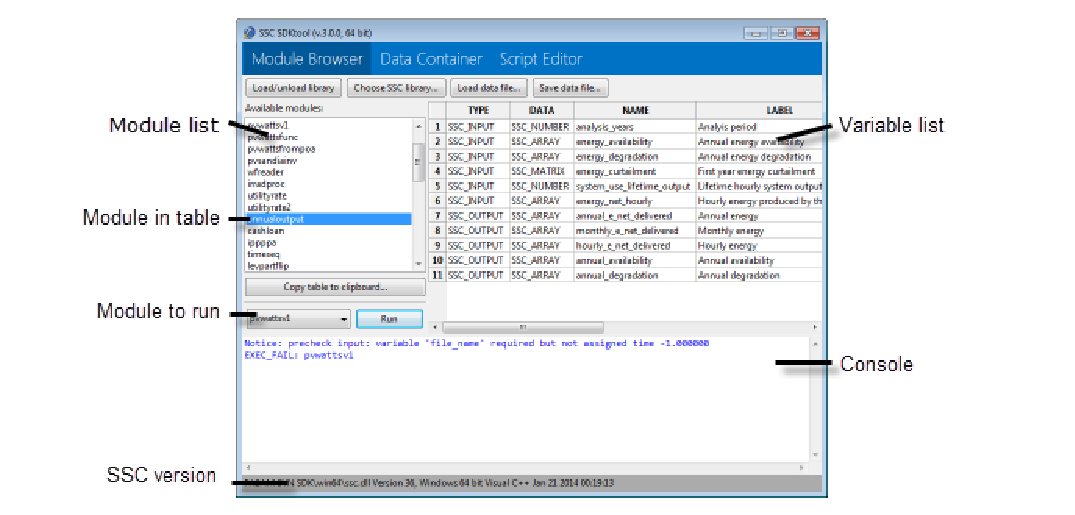
\includegraphics{modulebrowser}}
\end{center}
\caption{Module browser}
\label{fig_module_browser}
\end{figure}

The module browser displays the modules available in the SSC library. The module browser can:

\begin{itemize}
\item Display a list of available SSC modules.
\item Display a module's variables.
\item Copy a tab-delimited list of a module's variables to your computer's clipboard.
\item Run a single module using the variable values defined in the data container.
\end{itemize}

You can use the module browser as a reference while you are developing your model to help ensure that you assign values to all of the required input variables, and use the correct data types and units.

You can also use the module browser with the data container to manually set values of input variables and run modules individually. This might be useful for learning how a module works, or for troubleshooting your model's implementation of a module.

Module browser commands:
\begin{quote}
\begin{description}
\item[Load/unload library] Loads or unloads the current SSC library for troubleshooting. If a module does not run, you can try unloading and reloading the library.
\item[Choose SSC library] Displays a file dialog where you can choose and load the SSC library. Be sure to choose the correct library for your version of SDKtool.
\item[Load data file] Open a data file. (\texttt{.bdat}).
\item[Save data file] Save the variables in the data container to a data file. (\texttt{.bdat}).
\item[Copy table to clipboard] Copies the table of module variables as tab-delimited text to your computer's clipboard.
\item[Run] Runs the active module in the module browser. (You must select a module from the dropdown list before you click \textbf{Run}.)
\end{description}
\end{quote}

\subsection{Data Container}
\label{sec_data_container}

\begin{figure}
\begin{center}
\scalebox{0.95}{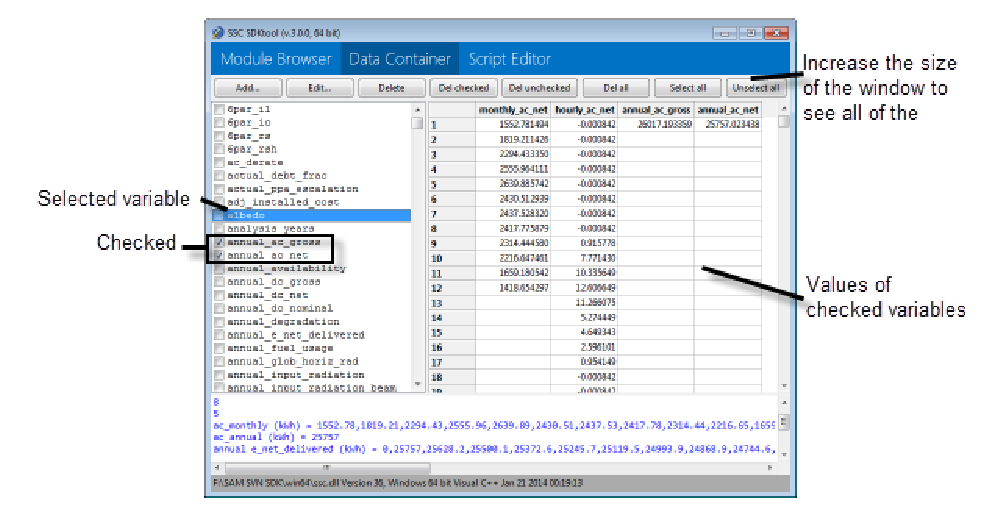
\includegraphics{datacontainer}}
\end{center}
\caption{Data container}
\label{fig_data_container}
\end{figure}

The data container displays a list of variables for the current set of simulations. When you run a module from the data browser, you must add input variables to the data container by hand using the \textbf{Add} and \textbf{Edit} buttons.

When you run modules from the script editor, the data container is automatically populated with variables from the script. You can use the data container commands for the following tasks:

\begin{itemize}
\item Add, edit, and remove variables from the data container.
\item Copy a tab-delimited list of variable names and values to your computer's clipboard.
\item Show graphs of time series data.
\end{itemize}

The data container commands act either on the selected variable indicated with a blue highlight, or on variables with a check mark. You may need to maximize the SDKtool window to see all of the command buttons:

\begin{quote}
\begin{description}
\item[Add] Add a variable to the data container. If you add a module's input variable to the data container, be sure to use the variable's exact name and data type as it appears in the module browser.
\item[Edit] Change the selected variable's name, data type, or value.
\item[Delete] Remove the selected variable from the data container.
\item[Del checked] Remove all variables with check marks from the data container.
\item[Del unchecked] Remove all variables without check marks from the data container.
\item[Del all] Delete all variables from the data container.
\item[Select all]  Check all variables in the data container. This command may take several seconds to complete.
\item[Unselect all] Clear check marks from all variables in the data container.
\item[Copy to clipboard] Copy the data container table as a tab-delimited list of selected variable names and their values to the clipboard.
\item[Show stats] Display a table of statistics for the selected variable, which must be of type \texttt{SSC\_ARRAY} with 8,760 values.
\item[Timeseries graph] Display time series and statistical graphs of variables with check marks, which must be of type \texttt{SSC\_ARRAY} with 8,760 values.
\end{description}
\end{quote}

\notebox{If you manually add variables to the data container before running a script that does not use the variables, they will be deleted from the data container.}

\subsubsection{Data Files}
\label{sec_data_files}

You can save and open the contents of the data container in a data file (\texttt{.bdat}) using the \textbf{Save data file} and \textbf{Load data file} commands on the File menu. The data files use a binary format, and store all of the variables in the data container.

\subsubsection{Time Series Graphs and Statistical Tables}
\label{sec_timeseries_statistical}

When the data container includes hourly arrays with 8,760 values, you can display the hourly data and statistical summaries:

Select an hourly array and click \textbf{Show stats} to display a statistical summary of the array data in a table. You can export data from the monthly table by selecting it using your computer's copy-to-clipboard keyboard shortcut (Ctrl-C) in windows.

Check one or more hourly arrays and click \textbf{Timeseries graph} time series data and statistical summaries in graphs. You can export graph images and tables of graph data by right-clicking graphs and selecting commands in the shortcut menu.

See \S\ref{sec_sdktool_example_1} for an example.

\subsection{Script Editor}
\label{sec_script_editor}

\begin{figure}
\begin{center}
\scalebox{0.95}{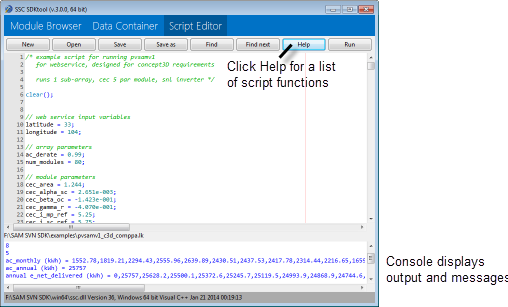
\includegraphics{scripteditor}}
\end{center}
\caption{Script editor}
\label{fig_script_editor}
\end{figure}

The script editor allows you to write, edit, and run scripts in LK Script to build and test models using the SSC modules. Documentation of LK Script is included in the SDK package in \texttt{lk\_guide.pdf}.

The script editor commands are:

\begin{quote}
\begin{description}
\item[New] Clear the current script from the script editor.
\item[Open]  (\textbf{Ctrl-O}) Open a script file (\texttt{.lk}).
\item[Save] (\textbf{Ctrl-S}) Save the current script file (\texttt{.lk}).
\item[Save as] Save the current script to a different file (\texttt{.lk}).
\item[Find] Find text in the current script.
\item[Find next] Find the next instance of text in the current script.
\item[Help] Display a list of script functions.
\item[Run] Run the current script.
\end{description}
\end{quote}

\subsection{SDKtool Example 1: Run a Module from the Module Browser}
\label{sec_sdktool_example_1}

The following example shows how to use the module browser to expore and run the \texttt{pvwattsv1} module. You can use the same steps to explore other simulation modules.

\notebox{As described in \S\ref{sec_module_browser}, the module browser can only run a single simulation module at a time. To combine modules to build a model, you can write a script as described in \S\ref{sec_sdktool_example_2}.}

As we saw in \S\ref{sec_modeling_systems}, the \texttt{pvwattsv1} simulation module reads data from a weather file and inputs from the data container that define the system's size, array orientation and type of tracking, and derating factor, and calculates values for the 1 by 8760 array storing the system's hourly electricity output over a single year.

To explore the \texttt{pvwattsv1} simulation module in the module browser:

\begin{enumerate}
\item Start SDKtool and be sure the correct SSC library is loaded as described in \S\ref{sec_sdktool_run}

\item In the \textbf{Module Browser}, click the \texttt{pvwattsv1} name to see a list of the module's variables. The inputs are of type \texttt{SSC\_INPUT}. Of the inputs, only a subset indicated by (\texttt{*}) are required and have no default value, as described in \S\ref{sec_def_const}. At a minimum, you must assign values to these variables to run the module.

\item In the drop-down list at the bottom of the window under the list of available modules, choose the \texttt{pvwatts1} module and click \textbf{Run}.

A message about the \texttt{file\_name} variable appears in the console. That is because \texttt{file\_name} is a required variable, but it does not yet have a value.

\item In the \textbf{Data Container}, click \textbf{Add}, and type "file\_name" for the variable name, assign it the \texttt{SSC\_STRING} data type, and click \textbf{file} to assign it the value of one of the TMY2 files included in the SDK Examples folder (for example, \textit{daggett.tm2}).

\item Next, add the remaining 5 required variables shown in the module browser to the data container, using the data type and units shown in the table. For example, \texttt{system\_size} should be \texttt{SSC\_NUMBER} with a value in kilowatts. Be sure to use variable names and data types that exactly match those in the module browser.

When you are finished, you should see a table similar to Table \ref{tab_pvwattsv1}. This is the model's data container, which so far contains the required input for the \texttt{pvwattsv1} simulation module.

\item In the \textbf{Module Browser}, click \textbf{Run} to run the module. 
\end{enumerate}

The data container should now show a table with all of the \texttt{pvwattsv1} module variables. You can edit and view the variable values:

\begin{itemize}

\item Use the check boxes to add or remove variables from the table. Double-click the variable's name to edit it (or select the variable and click \textbf{Edit}).

\item Display graphs of any array with 8,760 values. For example, to view the cell temperature and AC output variables, clear all of the check boxes, check the \texttt{tcell} and \texttt{ac} variables, and click \textbf{Time series graph}.

\item Display a table of statistical values for any variable with 8,760 values. For example, select the \texttt{poa} variable to show the plane-of-array irradiance minimum, maximum, total, mean, and monthly values, and click \textbf{Show stats}.

\notebox{To display the statistical summary of an hourly variable, select it by clicking its name in the list rather than checking it.}

\end{itemize}

\begin{table}
\begin{center}
\begin{tabular}{|l|c|c|c|c|c|}\hline
file\_name & system\_size & derate & track\_mode & azimuth & tilt\\
\hline
.../daggett.tm2 & 4 & 0.77 & 0 & 180 & 20\\
\hline\end{tabular}
\caption{The 6 required input variables for the pvwattsv1 module with their values}\label{tab_pvwattsv1}
\end{center}
\end{table}

\subsection{SDKtool Example 2: Build a Model in LK Script}
\label{sec_sdktool_example_2}

This example uses a script to run the \texttt{pvwattsv1} simulation module as we did in Example 1, and combine it with the \texttt{annualoutput} module to create a simple model that estiimates a PV system's annual output over a multi-year period.

Writing a script is a useful way to test your model before you implement it in C++ or another programming language. When you develop the model as a script in SDKtool, you can use the module browser and data container to help you troubleshoot your model within an environment designed specifically to run the modules. Once you get your model running as a script, you can easily translate it into another language.

Copy or cut and paste the script examples below into the SDKtool's script editor.

The first part of the script performs three tasks:

\begin{enumerate}
\item Assign values to the required input variables for \texttt{pvwattsv1}.
\item Run the module.
\item Display the total annual output.
\end{enumerate}

The next part of the script uses the system's AC output calculated by the \texttt{pvwattsv1} module to estimate the system's total annual output over multiple years:

\begin{enumerate}
\item Assign values to the required input variables for \texttt{annualoutput}.
\item Run the module.
\item Display the year-by-year output.
\end{enumerate}

The \texttt{pvwattsv1} module's required input variables are shown in Table \ref{tab_pvwattsv1}. The module browser shows each variable's data type, units, and any constraints.

\begin{verbatimtab}

// Create variables for the six pvwattsv1 module required inputs
weather_file = 'F:/SAM SDK/examples/daggett.tm2';
nameplate_capacity = 4; // DC kW
derating_factor = 0.77;
tracking = 0; // fixed
azimuth = 180; // due south
tilt = 20; // from horizontal

// Assign input values to the module inputs
var('file_name',weather_file);
var('system_size',nameplate_capacity);
var('derate',derating_factor);
var('track_mode',tracking);
var('azimuth',azimuth);
var('tilt',tilt);

// Run module
run('pvwattsv1');

// Get results
year_1_energy_total = var('ac_annual');
year_1_energy_hourly = var('ac');

sum_of_hourly = sum(year_1_energy_hourly);

// Display results
outln("Year 1 output: " + sprintf('%,',to_int(year_1_energy_total)) 
                                  + " kWh");
outln("  as sum of hourly output: " + sprintf('%,',to_int(sum_of_hourly)) 
                                              + " Wh");
outln();

\end{verbatimtab}

The next part of the script uses the \texttt{annualoutput} module to calculate the system's output over a multi-year period. It has the six required inputs shown in Table \ref{tab_annualoutput}.

\begin{table}[ht]
\begin{center}
\begin{tabular}{lll}
Name & Data Type & Units \\
\hline
analysis\_years & \texttt{SSC\_NUMBER} & years \\
energy\_availability & \texttt{SSC\_ARRAY} & \% \\
energy\_degradation & \texttt{SSC\_ARRAY} & \% \\
energy\_curtailment & \texttt{SSC\_MATRIX} & none \\
system\_use\_lifetime\_output & \texttt{SSC\_NUMBER} &  none \\
energy\_net\_hourly & \texttt{SSC\_ARRAY} &  kW \\
\end{tabular}
\caption{The six required input variables for the \texttt{annualoutput} module}\label{tab_annualoutput}
\end{center}
\end{table}

The module browser does not provide information about the size of the \texttt{energy\_availability} and \texttt{energy\_degradation} arrays, or the \texttt{energy\_curtailment} matrix. We can refer to the SAM user interface to explore those variables further. SAM displays them on the Performance Adjustment page as shown in Table \ref{tab_performance_adjustment}.

 \begin{table}[ht]
\begin{center}
\begin{tabular}{lll}
Variable & Name in SAM & Size \\
\hline
energy\_availability & Percent of annual output & 1x1 to 1x50 \\
energy\_degradation & Year-to-year decline in output & 1x1 to 1x50 \\
energy\_curtailment & Hourly Factors & 24x12 \\
\end{tabular}
\caption{Information from the SAM user interface about the inputs to \texttt{annualoutput}}\label{tab_performance_adjustment}
\end{center}
\end{table}

The SAM user interface allows the \textbf{Percent of annual output} (\texttt{energy\_availability}) and \textbf{Year-to-year decline in output} (\texttt{energy\_degradation}) variables to be specified either as a single value or as an "annual schedule." The input table for the annual schedule has a maximum size of 50 rows, indicating the maximum size of the arrays. If the array has a single value, \texttt{annualoutput} applies that value to each year in the analysis period. This behavior is described in SAM's Help system.

The 24 columns and 12 rows of the input table for the \textbf{Hourly Factors} variable shows the dimensions of the (\texttt{energy\_curtailment}) matrix.

\begin{verbatimtab}

// Create variables for the annualoutput module required inputs
// system_output already defined above
analysis_period = 25;
availability = [98];
degradation = [0.05];
curtailment = [ [1,1,1,1,1,1,1,1,1,1,1,1,1,1,1,1,1,1,1,1,1,1,1,1,],
                [1,1,1,1,1,1,1,1,1,1,1,1,1,1,1,1,1,1,1,1,1,1,1,1,],
                [1,1,1,1,1,1,1,1,1,1,1,1,1,1,1,1,1,1,1,1,1,1,1,1,],
                [1,1,1,1,1,1,1,1,1,1,1,1,1,1,1,1,1,1,1,1,1,1,1,1,],
                [1,1,1,1,1,1,1,1,1,1,1,1,1,1,1,1,1,1,1,1,1,1,1,1,],
                [1,1,1,1,1,1,1,1,1,1,1,1,1,1,1,1,1,1,1,1,1,1,1,1,],
                [1,1,1,1,1,1,1,1,1,1,1,1,1,1,1,1,1,1,1,1,1,1,1,1,],
                [1,1,1,1,1,1,1,1,1,1,1,1,1,1,1,1,1,1,1,1,1,1,1,1,],
                [1,1,1,1,1,1,1,1,1,1,1,1,1,1,1,1,1,1,1,1,1,1,1,1,],
                [1,1,1,1,1,1,1,1,1,1,1,1,1,1,1,1,1,1,1,1,1,1,1,1,],
                [1,1,1,1,1,1,1,1,1,1,1,1,1,1,1,1,1,1,1,1,1,1,1,1,],
                [1,1,1,1,1,1,1,1,1,1,1,1,1,1,1,1,1,1,1,1,1,1,1,1,] ];
hourly_mode = 0;

// Assign input values to the module inputs
var('analysis_years', analysis_period);
var('energy_availability', availability);
var('energy_degradation', degradation);
var('energy_curtailment', curtailment);
var('system_use_lifetime_output', hourly_mode);
var('energy_net_hourly', year_1_energy_hourly);

// Run module
run('annualoutput');

yearly_energy = var('annual_e_net_delivered');

for ( i = 1; i <= analysis_period; i++)
{
  outln("Year " + i + " output: " + sprintf('%,',to_int(yearly_energy[i])) 
                                            + ( " kWh"));
}


\end{verbatimtab}

\section{Language Interfaces}
\label{sec_language_interfaces}

The SSC software development kit (SDK) includes interfaces (or wrappers) for using SSC directly from programming languages other than its native C language interface.  This section describes each language interface and requirements, as well any limitations in functionality compared with the native C interface.

Each language interface comes with a set of readme and example files that you should refer to in addition to the descriptions below to set up your system to run SSC with a language interface.

\subsection{Generating Code from the SAM User Interface}

The desktop version of the System Advisor Model (SAM) can automatically export input data from each case in the project file to ready-to-run code in the following languages:

\begin{itemize}
\item LK for SDKtool will run from the SDKtool script editor.
\item C
\item MATLAB
\item Python 2 or 3
\item Java
\item PHP 5 or 7
\item C\#
\item VBA
\end{itemize}

For instructions on how to export code from SAM, see the \emph{Software Development Kit} topic in SAM's Help system. 

\subsection{Python}

The Python language interface has been tested on Windows with the ActivePython distribution, and on the Linux and OSX native Python packages.

The Python API is defined in the \texttt{sscapi.py} source file included in the SDK.  The file includes example code if it is invoked as the main source program.

\notebox{In the PySSC class constructor, a \emph{Ctypes} object is created by referencing the \texttt{ssc.dll} dynamic library.  It is up to the user to modify the file name and/or path of this library to be appropriate for the operating system and platform.}

The structure of SSC API calls in Python is slightly different from the C interface because in Python, an instance of the PySSC class must be created first.  Example:

\begin{verbatimtab}[4]
	ssc = PySSC()
	dat = ssc.data_create()

	ssc.data_set_string(dat, 'file_name', 'daggett.tm2')
	ssc.data_set_number(dat, 'system_size', 4)
	ssc.data_set_number(dat, 'derate', 0.77)
	ssc.data_set_number(dat, 'track_mode', 0)
	ssc.data_set_number(dat, 'azimuth', 180)
	ssc.data_set_number(dat, 'tilt_eq_lat', 1)

	# run PV system simulation
	mod = ssc.module_create("pvwattsv1")

	if ssc.module_exec(mod, dat) == 0:
		print 'PVWatts V1 simulation error'
		idx = 1
		msg = ssc.module_log(mod, 0)
		while (msg != None):
			print '\t: ' + msg
			msg = ssc.module_log(mod, idx)
			idx = idx + 1
	else:
		ann = 0
		ac = ssc.data_get_array(dat, "ac")
		for i in range(len(ac)):
			ac[i] = ac[i]/1000
			ann += ac[i]
		print 'PVWatts V1 Simulation ok, e_net (annual kW)=', ann
		ssc.data_set_array(dat, "e_with_system", ac) # copy over ac

	ssc.module_free(mod)

	ssc.data_free( dat )
\end{verbatimtab}

Notice that the structure of creating and freeing data containers and modules is identical to the C language API, except that the functions are members of the PySSC class.  For more information, see the \texttt{sscapi.py} source file for additional examples and usage cases.

\subsection{MATLAB}

MATLAB is a numerical computing language that is widely used for data processing, algorithm development, and plotting.  It is a proprietary product that is available on OSX, Linux, and Windows.  

The built-in MATLAB \emph{foreign function interface (FFI)} library routines that are used to interface to SSC require a C compiler to preprocess the SSC header file. Some versions of MATLAB include a C compiler such as LCC installed by default, while others may require that one to be installed separately.  See \url{http://www.mathworks.com/support/compilers/R2012b/win64.html} for more information.

The MATLAB environment should also be configured to recognize the path containing the SSC MATLAB files.

The MATLAB language interface automatically attempts to detect the platform and load the correct SSC dynamic library.  You must ensure that the \texttt{sscapi.h} C language header file can be located by MATLAB, as well as the library appropriate for your system.  

For additional information, see the MATLAB code examples supplied with the SSC SDK, as well as the content of the \texttt{ssccall.m} file itself.

The SSC API is provided in the \texttt{ssccall.m} M-file.  The interface provides a single MATLAB function called \texttt{ssccall(...)} that accepts different parameter arguments to invoke the various SSC library calls.  The example below shows how to setup and run the \emph{pvwattsv1} module from MATLAB.

\begin{verbatimtab}[4]
ssccall('load');

% create a data container to store all the variables
data = ssccall('data_create');

% setup the system parameters
ssccall('data_set_string', data, 'file_name', 'abilene.tm2');
ssccall('data_set_number', data, 'system_size', 4);
ssccall('data_set_number', data, 'derate', 0.77);
ssccall('data_set_number', data, 'track_mode', 0);
ssccall('data_set_number', data, 'tilt', 30);
ssccall('data_set_number', data, 'azimuth', 180);

% create the PVWatts module
module = ssccall('module_create', 'pvwattsv1');

% run the module
ok = ssccall('module_exec', module, data);
if ok,
    % if successful, retrieve the hourly AC generation data and print
    % annual kWh on the screen
    ac = ssccall('data_get_array', data, 'ac');
    disp(sprintf('pvwatts: %.2f kWh',sum(ac)/1000.0));
else
    % if it failed, print all the errors
    disp('pvwattsv1 errors:');
    ii=0;
    while 1,
        err = ssccall('module_log', module, ii);
        if strcmp(err,''),
            break;
        end
        disp( err );
        ii=ii+1;
    end
end

% free the PVWatts module that we created
ssccall('module_free', module);

% release the data container and all of its variables
ssccall('data_free', data);

% unload the library
ssccall('unload');
\end{verbatimtab}


\subsection{C\# and .NET}

The C\# language interface provides direct access to the SSC library from the Microsoft .NET software environment.  C\# is an object-oriented garbage-collected language that is compiled typically to an intermediate bytecode that is executed in a managed environment by the bytecode interpreter engine.  Objects and memory are directly managed by the interpreter, relieving programmers of the burdens of detailed memory management.  However, since SSC is implemented at its core in a native compiled machine code library, care must be taken by the typical C\# programmer to ensure that the interface to the unmanaged SSC library is properly utilized.

The C\# SSC language interface is provided as a single source file called \texttt{SSC.cs}.  This file contains direct invocation mappings to the unmanaged C library API, as well as an easy-to-use wrapper around the low-level function calls.  This API has been tested using Visual Studio 2012 .NET on Win32 and x64.  .NET implementations on other platforms such as Mono have not been tested.

To call the SSC library from C\#, include the \texttt{SSC.cs} file in your .NET project in Visual Studio. For each opaque data pointer type in the SSC native C API, there is a similarly named C\# class within the SSC namespace.  See the example below on how to create a data container and module to run PVWatts.  Additional examples of the other SSC API functions using the C\# wrapper classes is available in the included test program in the SDK.

\begin{verbatimtab}[4]
private void btnPVWatts_Click(object sender, EventArgs e)
{
	txtData.Clear();

	SSC.Data data = new SSC.Data();

	data.SetString("file_name", "abilene.tm2");
	data.SetNumber("system_size", 4.0f);
	data.SetNumber("derate", 0.77f);
	data.SetNumber("track_mode", 0);
	data.SetNumber("tilt", 20);
	data.SetNumber("azimuth", 180);

	SSC.Module mod = new SSC.Module("pvwattsv1");

	if (mod.Exec(data))
	{
		float tot = data.GetNumber("ac_annual");
		float[] ac = data.GetArray("ac_monthly");
		for (int i = 0; i < ac.Count(); i++)
			txtData.AppendText("[" + i + "]: " + ac[i] + " kWh\n");
		txtData.AppendText("AC total: " + tot + "\n");
		txtData.AppendText("PVWatts test OK\n");
	}
	else
	{
		int idx = 0;
		String msg;
		int type;
		float time;
		while (mod.Log(idx, out msg, out type, out time))
		{
			String stype = "NOTICE";
			if (type == SSC.API.WARNING) stype = "WARNING";
			else if (type == SSC.API.ERROR) stype = "ERROR";

			txtData.AppendText("[ " + stype + " at time:" + time + " ]: " 
                               + msg + "\n");
			idx++;
		}

		txtData.AppendText("PVWatts example failed\n");
	}
}


\end{verbatimtab}

\notebox{The SSC C\# class library is designed to properly handle allocation and freeing of underlying native SSC data types.  However, due to the nature of the .NET runtime environment's garbage collector, it may appear that SSC objects are not freed right away.  While it is possible to invoke the garbage collector manually, it is generally not recommended to do so by the Visual Studio documentation.}

For more information, consult the \texttt{SSC.cs} source file, as well as the example Visual Studio project provided with the SDK.

\subsection{Java}

The Java interface to SSC utilizes the low-level Java Native Interface (JNI) specification to directly access the SSC library.  The JNI wrapper consists of a C source file \texttt{jssc.c} that wraps the SSC native C language API into JNI methods that can be compiled and loaded by the Java Virtual Machine (JVM) at runtime.  The source code for the JNI wrapper is included in the SDK, as well as a more programmer-friendly high-level Java \texttt{SSC} class that invokes the JNI layer.

The JNI interface marshals opaque C pointers as the 64-bit \texttt{jlong} data type, ensuring compatibility in both 32 and 64 bit implementations.

Compiling the JNI interface layer requires a C compiler and the Java SDK (for the JNI header files).  The example included with the SSC SDK was tested using the freely downloadable MinGW gcc compiler on 32-bit Windows (\texttt{https://www.mingw.org}), and the Java JDK 1.7.  Refer to the \texttt{README.txt} in the \texttt{[sdk]/languages/java/} folder for specific information on compiling the JNI interface layers for your particular SDK runtime environment.

Once the JNI wrapper library has been compiled for your particular JDK version, the PVWatts example can be invoked from within Java as below:

\begin{verbatimtab}[4]

public class SSC_Java_Example {
   
    public static void main(String[] args)
    {
        System.loadLibrary("sscapiJNI32");
		
        SSC sscobj = new SSC("pvwattsv1");

        sscobj.Set_String("file_name", "abilene.tm2" );
        sscobj.Set_Number("system_size", 4.0f );
        sscobj.Set_Number("derate", 0.77f );
        sscobj.Set_Number("track_mode", 0 );
        sscobj.Set_Number("tilt", 20 );
        sscobj.Set_Number("azimuth", 180 );
        
		if ( sscobj.Exec() )
        {
            float[] ac = sscobj.Get_Array( "ac" );
            float sum = 0;
            for( int i=0;ac.length;i++)
            {
                sum += ac[i];
            }
            System.out.println("ac total: " + sum);
            System.out.println("PVWatts example passed");
        }
        else
        {
            System.out.println("PVWatts example failed");
        }
    }    
}

\end{verbatimtab}

For more information on utilizing the Java language layer, consult Java code examples provided in the SDK.  


\subsection{PHP}

PHP: Hypertext Preprocessor (PHP) is a popular server-side scripting language designed for creating dynamic web pages.  Calling SSC from PHP requires you to compile and configure a PHP extension whose source code is provided in \texttt{sscphp.c} as part of the SSC SDK.  You need to have the PHP header files installed on your system that match the version of PHP you will be running.  The extension has been tested with PHP 5.4 on Slackware 14.1 and recent versions of Red Hat Enterprise Linux.

\begin{enumerate}
\item Compile the PHP extension.  The first line of the \texttt{Makefile} sets the path to the PHP header files, which defaults to \texttt{/usr/include/php}.  You may need to edit this for your specific system configuration.
\begin{verbatimtab}[4]
$ cd languages/php
$ cp ../../sscapi.h .
$ cp ../../linux64/ssc.so .
$ make
\end{verbatimtab}
Upon success, a new dynamic library \texttt{sscphp.so} will be created that can be loaded into PHP as an extension.
\item Configure PHP to load the extension by editing the \texttt{php.ini} file.  On Slackware Linux, this can be found in \texttt{/etc/httpd/php.ini}.  Add a line in the extensions section:
\begin{verbatimtab}[4]
extension=<path-to-ssc-sdk>/languages/php/sscphp.so
\end{verbatimtab}
\item At the shell, test that the module is loaded and working:
\begin{verbatimtab}[4]
$ php -r "echo sscphp_build_info();"
Unix 64 bit GNU/C++ Jun 2 2015 14:03:40
\end{verbatimtab}
If all is well, you should see detailed SSC build information printed on the console as above.
\item To run PHP scripts calling SSC from web pages served by the apache web server, you may need to restart the \texttt{httpd} service.  On Slackware:
\begin{verbatimtab}[4]
$ apachectl restart
\end{verbatimtab}
\end{enumerate}

The SDK package includes source code for a basic PVWatts Version 5 calculator web page. To set it up on a Linux system:
\begin{enumerate}
\item Copy \texttt{pvwatts.php}, \texttt{down-arrow.png}, and \texttt{jquery.searchabledropdown-1.0.8.min.js} to your HTML folder, typically \texttt{\textasciitilde/public\_html}.
\item Create a subfolder folder \texttt{ \textasciitilde/public\_html/weather}, and copy several SAM CSV formatted weather data files to this folder.  
\notebox{You can download the default SAM solar resource dataset, including all US TMY2/TMY3 files, and 360 international TMYs, by downloading and installing SAM (http://sam.nrel.gov).  The CSV solar resource files are located in 
\texttt{c:\textbackslash SAM\textbackslash <version>\textbackslash solar\_resource}.}

\item Point your web browser to \texttt{http://localhost/\textasciitilde<username>/pvwatts.php}.
\end{enumerate}


\begin{figure}[h]
\begin{center}
\scalebox{0.65}{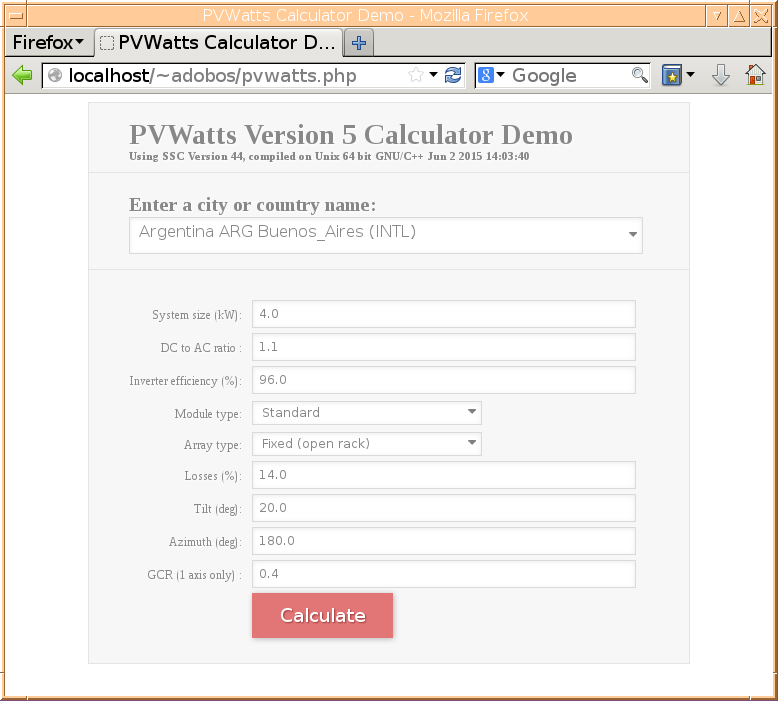
\includegraphics{pvwattsweb}}
\end{center}
\caption{Example PVWatts Version 5 Calculator PHP web page}
\label{fig_pvwatts_php}
\end{figure}

The portion of \texttt{pvwatts.php} that calls the SSC library is included below for reference.  

The PHP API very closely follows the native C API.  

The only differences are that \texttt{sscphp\_module\_var\_info(...)} and \texttt{sscphp\_module\_entry(...)} return PHP associative arrays containing the various fields that are normally accessed via the \texttt{ssc\_info\_*(...)} and \texttt{ssc\_entry\_*(...)} functions in the native API.

\begin{verbatimtab}[4]
	$dat = sscphp_data_create();	
	sscphp_data_set_string( $dat, "solar_resource_file", $wf );
	sscphp_data_set_number( $dat, "system_capacity", $size );
	sscphp_data_set_number( $dat, "module_type", $module );
	sscphp_data_set_number( $dat, "dc_ac_ratio", $dcacratio );
	sscphp_data_set_number( $dat, "inv_eff", $inveff );
	sscphp_data_set_number( $dat, "losses", $losses );
	sscphp_data_set_number( $dat, "array_type", $array );
	sscphp_data_set_number( $dat, "tilt", $tilt );
	sscphp_data_set_number( $dat, "azimuth", $azimuth );
	sscphp_data_set_number( $dat, "gcr", $gcr );
	sscphp_data_set_number( $dat, "adjust:constant", 0 );
	
	$mod = sscphp_module_create( "pvwattsv5" );
	if ( sscphp_module_exec( $mod, $dat ) )
	{
		$annual = sscphp_data_get_number( $dat, "annual_energy" );
		$monthly = sscphp_data_get_array( $dat, "monthly_energy" );
		$solrad = sscphp_data_get_array( $dat, "solrad_monthly" );
		$latitude = sscphp_data_get_number( $dat, "lat" );
		$longitude = sscphp_data_get_number( $dat, "lon" );
		$ok = true;
	}
	else
	{
		$index = 0;
		while ($err = sscphp_module_log( $mod, $index++ ) )
		{
			echo "$err<br>\n";
		}
	}	
	sscphp_module_free( $mod );
	sscphp_data_free( $dat );
\end{verbatimtab}


\section{C API Reference}\label{sec_api_ref}\hypertarget{sscapi_8h}{\subsection{sscapi.\-h File Reference}
\label{sscapi_8h}\index{sscapi.\-h@{sscapi.\-h}}
}


S\-S\-C\-: S\-A\-M Simulation Core.  


\subsubsection*{Macros}
\begin{DoxyCompactItemize}
\item 
\hypertarget{sscapi_8h_a41d524158813079fff1118377604a80b}{\#define {\bfseries S\-S\-C\-E\-X\-P\-O\-R\-T}}\label{sscapi_8h_a41d524158813079fff1118377604a80b}

\end{DoxyCompactItemize}
\begin{Indent}{\bf Data types\-:}\par
{\em Possible data types for variables in an ssc\-\_\-data\-\_\-t\-: }\begin{DoxyCompactItemize}
\item 
\hypertarget{sscapi_8h_abcf40c59544491ea45523ad3ce71e0ca}{\#define {\bfseries S\-S\-C\-\_\-\-I\-N\-V\-A\-L\-I\-D}~0}\label{sscapi_8h_abcf40c59544491ea45523ad3ce71e0ca}

\item 
\hypertarget{sscapi_8h_a7bdd11c9271bd1fa6177982a63df48fe}{\#define {\bfseries S\-S\-C\-\_\-\-S\-T\-R\-I\-N\-G}~1}\label{sscapi_8h_a7bdd11c9271bd1fa6177982a63df48fe}

\item 
\hypertarget{sscapi_8h_a78eee76ae837c41241907330a98c5288}{\#define {\bfseries S\-S\-C\-\_\-\-N\-U\-M\-B\-E\-R}~2}\label{sscapi_8h_a78eee76ae837c41241907330a98c5288}

\item 
\hypertarget{sscapi_8h_a39f84e7c07eb2d6f9cfededa992fdf1a}{\#define {\bfseries S\-S\-C\-\_\-\-A\-R\-R\-A\-Y}~3}\label{sscapi_8h_a39f84e7c07eb2d6f9cfededa992fdf1a}

\item 
\hypertarget{sscapi_8h_af2e80030586871134577f9ea5a941701}{\#define {\bfseries S\-S\-C\-\_\-\-M\-A\-T\-R\-I\-X}~4}\label{sscapi_8h_af2e80030586871134577f9ea5a941701}

\item 
\hypertarget{sscapi_8h_a2c360d77ec8cca52f1848ec230700530}{\#define {\bfseries S\-S\-C\-\_\-\-T\-A\-B\-L\-E}~5}\label{sscapi_8h_a2c360d77ec8cca52f1848ec230700530}

\end{DoxyCompactItemize}
\end{Indent}
\begin{Indent}{\bf Variable types\-:}\par
\begin{DoxyCompactItemize}
\item 
\hypertarget{sscapi_8h_a37c2de15c5bfe5e9fe89a2c41b8c23f2}{\#define {\bfseries S\-S\-C\-\_\-\-I\-N\-P\-U\-T}~1}\label{sscapi_8h_a37c2de15c5bfe5e9fe89a2c41b8c23f2}

\item 
\hypertarget{sscapi_8h_ac1567d5f42c5f5be4b5990679f810544}{\#define {\bfseries S\-S\-C\-\_\-\-O\-U\-T\-P\-U\-T}~2}\label{sscapi_8h_ac1567d5f42c5f5be4b5990679f810544}

\item 
\hypertarget{sscapi_8h_af2652950d87e4717878e75dc58de8a07}{\#define {\bfseries S\-S\-C\-\_\-\-I\-N\-O\-U\-T}~3}\label{sscapi_8h_af2652950d87e4717878e75dc58de8a07}

\end{DoxyCompactItemize}
\end{Indent}
\begin{Indent}{\bf Action/notification types that can be sent to a handler function\-:}\par
{\em S\-S\-C\-\_\-\-L\-O\-G\-: Log a message in the handler. f0\-: (int)message type, f1\-: time, s0\-: message text, s1\-: unused. S\-S\-C\-\_\-\-U\-P\-D\-A\-T\-E\-: Notify simulation progress update. f0\-: percent done, f1\-: time, s0\-: current action text, s1\-: unused. }\begin{DoxyCompactItemize}
\item 
\hypertarget{sscapi_8h_add30e629a1f45f721fe51e0f6be08752}{\#define {\bfseries S\-S\-C\-\_\-\-L\-O\-G}~0}\label{sscapi_8h_add30e629a1f45f721fe51e0f6be08752}

\item 
\hypertarget{sscapi_8h_a0a1242ee7a03bba4b635f0a5064b76b0}{\#define {\bfseries S\-S\-C\-\_\-\-U\-P\-D\-A\-T\-E}~1}\label{sscapi_8h_a0a1242ee7a03bba4b635f0a5064b76b0}

\end{DoxyCompactItemize}
\end{Indent}
\begin{Indent}{\bf Message types\-:}\par
\begin{DoxyCompactItemize}
\item 
\hypertarget{sscapi_8h_a34adbabba29846c604dbef083b3c541c}{\#define {\bfseries S\-S\-C\-\_\-\-N\-O\-T\-I\-C\-E}~1}\label{sscapi_8h_a34adbabba29846c604dbef083b3c541c}

\item 
\hypertarget{sscapi_8h_a872c257a664d5cc7f52e4c3b4a59783e}{\#define {\bfseries S\-S\-C\-\_\-\-W\-A\-R\-N\-I\-N\-G}~2}\label{sscapi_8h_a872c257a664d5cc7f52e4c3b4a59783e}

\item 
\hypertarget{sscapi_8h_adf6646aa7c56ee16dd8b283e88005324}{\#define {\bfseries S\-S\-C\-\_\-\-E\-R\-R\-O\-R}~3}\label{sscapi_8h_adf6646aa7c56ee16dd8b283e88005324}

\end{DoxyCompactItemize}
\end{Indent}
\subsubsection*{Typedefs}
\begin{DoxyCompactItemize}
\item 
typedef void $\ast$ \hyperlink{sscapi_8h_a082e17260ab55ccb945bcabd4509f439}{ssc\-\_\-data\-\_\-t}
\item 
typedef float \hyperlink{sscapi_8h_aed2c6c08a4d87fc653895a27065b5c8d}{ssc\-\_\-number\-\_\-t}
\item 
typedef int \hyperlink{sscapi_8h_a8416be1f3d7e7d4457bf37e657277575}{ssc\-\_\-bool\-\_\-t}
\item 
typedef void $\ast$ \hyperlink{sscapi_8h_a0f778c7e3611dfc2ba01e5bd89979f80}{ssc\-\_\-entry\-\_\-t}
\item 
typedef void $\ast$ \hyperlink{sscapi_8h_adf8d62c898e485fc7440d3ed2fb0d87c}{ssc\-\_\-module\-\_\-t}
\item 
typedef void $\ast$ \hyperlink{sscapi_8h_aff18f3d1ec484009b88a779dcb69d456}{ssc\-\_\-info\-\_\-t}
\item 
typedef void $\ast$ \hyperlink{sscapi_8h_a64a6b436524349ccf0a77b56b2cf4e9d}{ssc\-\_\-handler\-\_\-t}
\end{DoxyCompactItemize}
\subsubsection*{Functions}
\begin{DoxyCompactItemize}
\item 
S\-S\-C\-E\-X\-P\-O\-R\-T int \hyperlink{sscapi_8h_a4460dd3f2316afa8a766769445e9fcd6}{ssc\-\_\-version} ()
\item 
S\-S\-C\-E\-X\-P\-O\-R\-T const char $\ast$ \hyperlink{sscapi_8h_ab34ddddf0832ff80d36c08af415fcf61}{ssc\-\_\-build\-\_\-info} ()
\item 
S\-S\-C\-E\-X\-P\-O\-R\-T \hyperlink{sscapi_8h_a082e17260ab55ccb945bcabd4509f439}{ssc\-\_\-data\-\_\-t} \hyperlink{sscapi_8h_ac9f368730a0da3c79169cd6d3eef8f0b}{ssc\-\_\-data\-\_\-create} ()
\item 
S\-S\-C\-E\-X\-P\-O\-R\-T void \hyperlink{sscapi_8h_acc9123254cfd9b1483a34a840ba66f3f}{ssc\-\_\-data\-\_\-free} (\hyperlink{sscapi_8h_a082e17260ab55ccb945bcabd4509f439}{ssc\-\_\-data\-\_\-t} p\-\_\-data)
\item 
S\-S\-C\-E\-X\-P\-O\-R\-T void \hyperlink{sscapi_8h_adc28c6035c08ce6f88d5e228b3d3cd25}{ssc\-\_\-data\-\_\-clear} (\hyperlink{sscapi_8h_a082e17260ab55ccb945bcabd4509f439}{ssc\-\_\-data\-\_\-t} p\-\_\-data)
\item 
S\-S\-C\-E\-X\-P\-O\-R\-T void \hyperlink{sscapi_8h_a5044cd17abb621f4549c6fd0aab77277}{ssc\-\_\-data\-\_\-unassign} (\hyperlink{sscapi_8h_a082e17260ab55ccb945bcabd4509f439}{ssc\-\_\-data\-\_\-t} p\-\_\-data, const char $\ast$name)
\item 
S\-S\-C\-E\-X\-P\-O\-R\-T int \hyperlink{sscapi_8h_ab6598d213b423fe7c3b85071119f4cb0}{ssc\-\_\-data\-\_\-query} (\hyperlink{sscapi_8h_a082e17260ab55ccb945bcabd4509f439}{ssc\-\_\-data\-\_\-t} p\-\_\-data, const char $\ast$name)
\item 
S\-S\-C\-E\-X\-P\-O\-R\-T const char $\ast$ \hyperlink{sscapi_8h_ad499cfe8696e1f704d968b50d3ab36b1}{ssc\-\_\-data\-\_\-first} (\hyperlink{sscapi_8h_a082e17260ab55ccb945bcabd4509f439}{ssc\-\_\-data\-\_\-t} p\-\_\-data)
\item 
S\-S\-C\-E\-X\-P\-O\-R\-T const char $\ast$ \hyperlink{sscapi_8h_a56b8a556bfe81c4f65fa2f3c41b5db31}{ssc\-\_\-data\-\_\-next} (\hyperlink{sscapi_8h_a082e17260ab55ccb945bcabd4509f439}{ssc\-\_\-data\-\_\-t} p\-\_\-data)
\item 
S\-S\-C\-E\-X\-P\-O\-R\-T \hyperlink{sscapi_8h_a0f778c7e3611dfc2ba01e5bd89979f80}{ssc\-\_\-entry\-\_\-t} \hyperlink{sscapi_8h_acb6e7a1f9ac26d3160fc849754a38627}{ssc\-\_\-module\-\_\-entry} (int index)
\item 
S\-S\-C\-E\-X\-P\-O\-R\-T const char $\ast$ \hyperlink{sscapi_8h_a785b1e08e248478ee792ac945bd1eb31}{ssc\-\_\-entry\-\_\-name} (\hyperlink{sscapi_8h_a0f778c7e3611dfc2ba01e5bd89979f80}{ssc\-\_\-entry\-\_\-t} p\-\_\-entry)
\item 
S\-S\-C\-E\-X\-P\-O\-R\-T const char $\ast$ \hyperlink{sscapi_8h_a86977139c320479baf3b4762513a8f6d}{ssc\-\_\-entry\-\_\-description} (\hyperlink{sscapi_8h_a0f778c7e3611dfc2ba01e5bd89979f80}{ssc\-\_\-entry\-\_\-t} p\-\_\-entry)
\item 
S\-S\-C\-E\-X\-P\-O\-R\-T int \hyperlink{sscapi_8h_a449e4d53d00830b7b85a1e88a99f078f}{ssc\-\_\-entry\-\_\-version} (\hyperlink{sscapi_8h_a0f778c7e3611dfc2ba01e5bd89979f80}{ssc\-\_\-entry\-\_\-t} p\-\_\-entry)
\item 
S\-S\-C\-E\-X\-P\-O\-R\-T \hyperlink{sscapi_8h_adf8d62c898e485fc7440d3ed2fb0d87c}{ssc\-\_\-module\-\_\-t} \hyperlink{sscapi_8h_a128141ac47daba53202b86a009e1cea7}{ssc\-\_\-module\-\_\-create} (const char $\ast$name)
\item 
S\-S\-C\-E\-X\-P\-O\-R\-T void \hyperlink{sscapi_8h_a55fb17057398f14de0f7a3fcba9d328e}{ssc\-\_\-module\-\_\-free} (\hyperlink{sscapi_8h_adf8d62c898e485fc7440d3ed2fb0d87c}{ssc\-\_\-module\-\_\-t} p\-\_\-mod)
\item 
S\-S\-C\-E\-X\-P\-O\-R\-T const \hyperlink{sscapi_8h_aff18f3d1ec484009b88a779dcb69d456}{ssc\-\_\-info\-\_\-t} \hyperlink{sscapi_8h_acfb10163d7b9bea42b2e444c2a5544ac}{ssc\-\_\-module\-\_\-var\-\_\-info} (\hyperlink{sscapi_8h_adf8d62c898e485fc7440d3ed2fb0d87c}{ssc\-\_\-module\-\_\-t} p\-\_\-mod, int index)
\item 
S\-S\-C\-E\-X\-P\-O\-R\-T int \hyperlink{sscapi_8h_a25c204af7a2c81d11d134a62702426b5}{ssc\-\_\-info\-\_\-var\-\_\-type} (\hyperlink{sscapi_8h_aff18f3d1ec484009b88a779dcb69d456}{ssc\-\_\-info\-\_\-t} p\-\_\-inf)
\item 
S\-S\-C\-E\-X\-P\-O\-R\-T int \hyperlink{sscapi_8h_ab2fde3d3031880da882aee086afc76b3}{ssc\-\_\-info\-\_\-data\-\_\-type} (\hyperlink{sscapi_8h_aff18f3d1ec484009b88a779dcb69d456}{ssc\-\_\-info\-\_\-t} p\-\_\-inf)
\item 
S\-S\-C\-E\-X\-P\-O\-R\-T const char $\ast$ \hyperlink{sscapi_8h_a92f71d2241b912330d2734ba63d6b85f}{ssc\-\_\-info\-\_\-name} (\hyperlink{sscapi_8h_aff18f3d1ec484009b88a779dcb69d456}{ssc\-\_\-info\-\_\-t} p\-\_\-inf)
\item 
S\-S\-C\-E\-X\-P\-O\-R\-T const char $\ast$ \hyperlink{sscapi_8h_a04113d80460294539d935c04ca8d8f36}{ssc\-\_\-info\-\_\-label} (\hyperlink{sscapi_8h_aff18f3d1ec484009b88a779dcb69d456}{ssc\-\_\-info\-\_\-t} p\-\_\-inf)
\item 
S\-S\-C\-E\-X\-P\-O\-R\-T const char $\ast$ \hyperlink{sscapi_8h_aafe4ecee010642fabc99b1591c0680f8}{ssc\-\_\-info\-\_\-units} (\hyperlink{sscapi_8h_aff18f3d1ec484009b88a779dcb69d456}{ssc\-\_\-info\-\_\-t} p\-\_\-inf)
\item 
S\-S\-C\-E\-X\-P\-O\-R\-T const char $\ast$ \hyperlink{sscapi_8h_a6e13987c293cb1044d893dee334daa5b}{ssc\-\_\-info\-\_\-meta} (\hyperlink{sscapi_8h_aff18f3d1ec484009b88a779dcb69d456}{ssc\-\_\-info\-\_\-t} p\-\_\-inf)
\item 
S\-S\-C\-E\-X\-P\-O\-R\-T const char $\ast$ \hyperlink{sscapi_8h_a988bfd5148b165f3f3fc9f9f0f021262}{ssc\-\_\-info\-\_\-group} (\hyperlink{sscapi_8h_aff18f3d1ec484009b88a779dcb69d456}{ssc\-\_\-info\-\_\-t} p\-\_\-inf)
\item 
S\-S\-C\-E\-X\-P\-O\-R\-T const char $\ast$ \hyperlink{sscapi_8h_a9ef2812e6f2c9b4a650c5e729f5c5ef5}{ssc\-\_\-info\-\_\-required} (\hyperlink{sscapi_8h_aff18f3d1ec484009b88a779dcb69d456}{ssc\-\_\-info\-\_\-t} p\-\_\-inf)
\item 
S\-S\-C\-E\-X\-P\-O\-R\-T const char $\ast$ \hyperlink{sscapi_8h_a1a5af0286399b099684fa0f09ec149cf}{ssc\-\_\-info\-\_\-constraints} (\hyperlink{sscapi_8h_aff18f3d1ec484009b88a779dcb69d456}{ssc\-\_\-info\-\_\-t} p\-\_\-inf)
\item 
S\-S\-C\-E\-X\-P\-O\-R\-T const char $\ast$ \hyperlink{sscapi_8h_ab895b6deba0be468250fc84ff027ed73}{ssc\-\_\-info\-\_\-uihint} (\hyperlink{sscapi_8h_aff18f3d1ec484009b88a779dcb69d456}{ssc\-\_\-info\-\_\-t} p\-\_\-inf)
\item 
S\-S\-C\-E\-X\-P\-O\-R\-T void \hyperlink{sscapi_8h_ad4c7c528bb268bd95e87c363c224a659}{ssc\-\_\-module\-\_\-exec\-\_\-set\-\_\-print} (int print)
\item 
S\-S\-C\-E\-X\-P\-O\-R\-T \hyperlink{sscapi_8h_a8416be1f3d7e7d4457bf37e657277575}{ssc\-\_\-bool\-\_\-t} \hyperlink{sscapi_8h_a360e90bdd0738c494c7992f15467268d}{ssc\-\_\-module\-\_\-exec\-\_\-simple} (const char $\ast$name, \hyperlink{sscapi_8h_a082e17260ab55ccb945bcabd4509f439}{ssc\-\_\-data\-\_\-t} p\-\_\-data)
\item 
S\-S\-C\-E\-X\-P\-O\-R\-T const char $\ast$ \hyperlink{sscapi_8h_ae13b12f038c0c491cda6dfda90152abb}{ssc\-\_\-module\-\_\-exec\-\_\-simple\-\_\-nothread} (const char $\ast$name, \hyperlink{sscapi_8h_a082e17260ab55ccb945bcabd4509f439}{ssc\-\_\-data\-\_\-t} p\-\_\-data)
\item 
S\-S\-C\-E\-X\-P\-O\-R\-T \hyperlink{sscapi_8h_a8416be1f3d7e7d4457bf37e657277575}{ssc\-\_\-bool\-\_\-t} \hyperlink{sscapi_8h_a76d8a523407f3c071a9cf22ad2935a41}{ssc\-\_\-module\-\_\-exec} (\hyperlink{sscapi_8h_adf8d62c898e485fc7440d3ed2fb0d87c}{ssc\-\_\-module\-\_\-t} p\-\_\-mod, \hyperlink{sscapi_8h_a082e17260ab55ccb945bcabd4509f439}{ssc\-\_\-data\-\_\-t} p\-\_\-data)
\item 
S\-S\-C\-E\-X\-P\-O\-R\-T \hyperlink{sscapi_8h_a8416be1f3d7e7d4457bf37e657277575}{ssc\-\_\-bool\-\_\-t} \hyperlink{sscapi_8h_a58968776ff9ba65e9ac1886a0bdcb8df}{ssc\-\_\-module\-\_\-exec\-\_\-with\-\_\-handler} (\hyperlink{sscapi_8h_adf8d62c898e485fc7440d3ed2fb0d87c}{ssc\-\_\-module\-\_\-t} p\-\_\-mod, \hyperlink{sscapi_8h_a082e17260ab55ccb945bcabd4509f439}{ssc\-\_\-data\-\_\-t} p\-\_\-data, \hyperlink{sscapi_8h_a8416be1f3d7e7d4457bf37e657277575}{ssc\-\_\-bool\-\_\-t}($\ast$pf\-\_\-handler)(\hyperlink{sscapi_8h_adf8d62c898e485fc7440d3ed2fb0d87c}{ssc\-\_\-module\-\_\-t}, \hyperlink{sscapi_8h_a64a6b436524349ccf0a77b56b2cf4e9d}{ssc\-\_\-handler\-\_\-t}, int action, float f0, float f1, const char $\ast$s0, const char $\ast$s1, void $\ast$user\-\_\-data), void $\ast$pf\-\_\-user\-\_\-data)
\item 
S\-S\-C\-E\-X\-P\-O\-R\-T const char $\ast$ \hyperlink{sscapi_8h_a595854e4dc9d1e10e7a36eb1715b55dc}{ssc\-\_\-module\-\_\-log} (\hyperlink{sscapi_8h_adf8d62c898e485fc7440d3ed2fb0d87c}{ssc\-\_\-module\-\_\-t} p\-\_\-mod, int index, int $\ast$item\-\_\-type, float $\ast$time)
\item 
S\-S\-C\-E\-X\-P\-O\-R\-T void \hyperlink{sscapi_8h_ad5d381c3a156fce3bd92f6810129d2b7}{\-\_\-\-\_\-ssc\-\_\-segfault} ()
\end{DoxyCompactItemize}
\begin{Indent}{\bf Assigning variable values.}\par
{\em The following functions do not take ownership of the data pointeres for arrays, matrices, and tables. A deep copy is made into the internal S\-S\-C engine. You must remember to free the table that you create to pass into \hyperlink{sscapi_8h_a8f86dcefe1ddcf1b4190a4ee415d14f2}{ssc\-\_\-data\-\_\-set\-\_\-table( )} for example. }\begin{DoxyCompactItemize}
\item 
S\-S\-C\-E\-X\-P\-O\-R\-T void \hyperlink{sscapi_8h_aa660663a8343fb2ddb7f7aa1d6a93205}{ssc\-\_\-data\-\_\-set\-\_\-string} (\hyperlink{sscapi_8h_a082e17260ab55ccb945bcabd4509f439}{ssc\-\_\-data\-\_\-t} p\-\_\-data, const char $\ast$name, const char $\ast$value)
\item 
S\-S\-C\-E\-X\-P\-O\-R\-T void \hyperlink{sscapi_8h_a42e160996afdef0ab4b3c085c253e364}{ssc\-\_\-data\-\_\-set\-\_\-number} (\hyperlink{sscapi_8h_a082e17260ab55ccb945bcabd4509f439}{ssc\-\_\-data\-\_\-t} p\-\_\-data, const char $\ast$name, \hyperlink{sscapi_8h_aed2c6c08a4d87fc653895a27065b5c8d}{ssc\-\_\-number\-\_\-t} value)
\item 
S\-S\-C\-E\-X\-P\-O\-R\-T void \hyperlink{sscapi_8h_a2a65f966686e481fc4f63803a968f3d4}{ssc\-\_\-data\-\_\-set\-\_\-array} (\hyperlink{sscapi_8h_a082e17260ab55ccb945bcabd4509f439}{ssc\-\_\-data\-\_\-t} p\-\_\-data, const char $\ast$name, \hyperlink{sscapi_8h_aed2c6c08a4d87fc653895a27065b5c8d}{ssc\-\_\-number\-\_\-t} $\ast$pvalues, int length)
\item 
S\-S\-C\-E\-X\-P\-O\-R\-T void \hyperlink{sscapi_8h_ae823313deeeb06e37ddf6dfaab17190f}{ssc\-\_\-data\-\_\-set\-\_\-matrix} (\hyperlink{sscapi_8h_a082e17260ab55ccb945bcabd4509f439}{ssc\-\_\-data\-\_\-t} p\-\_\-data, const char $\ast$name, \hyperlink{sscapi_8h_aed2c6c08a4d87fc653895a27065b5c8d}{ssc\-\_\-number\-\_\-t} $\ast$pvalues, int nrows, int ncols)
\item 
S\-S\-C\-E\-X\-P\-O\-R\-T void \hyperlink{sscapi_8h_a8f86dcefe1ddcf1b4190a4ee415d14f2}{ssc\-\_\-data\-\_\-set\-\_\-table} (\hyperlink{sscapi_8h_a082e17260ab55ccb945bcabd4509f439}{ssc\-\_\-data\-\_\-t} p\-\_\-data, const char $\ast$name, \hyperlink{sscapi_8h_a082e17260ab55ccb945bcabd4509f439}{ssc\-\_\-data\-\_\-t} table)
\end{DoxyCompactItemize}
\end{Indent}
\begin{Indent}{\bf Retrieving variable values.}\par
{\em The following functions return internal references to memory, and the returned string, array, matrix, and tables should not be freed by the user. }\begin{DoxyCompactItemize}
\item 
S\-S\-C\-E\-X\-P\-O\-R\-T const char $\ast$ \hyperlink{sscapi_8h_a118454db6d4080a623bc176db005c7b1}{ssc\-\_\-data\-\_\-get\-\_\-string} (\hyperlink{sscapi_8h_a082e17260ab55ccb945bcabd4509f439}{ssc\-\_\-data\-\_\-t} p\-\_\-data, const char $\ast$name)
\item 
S\-S\-C\-E\-X\-P\-O\-R\-T \hyperlink{sscapi_8h_a8416be1f3d7e7d4457bf37e657277575}{ssc\-\_\-bool\-\_\-t} \hyperlink{sscapi_8h_a2a815f31617dee3c96587fe2df6938ff}{ssc\-\_\-data\-\_\-get\-\_\-number} (\hyperlink{sscapi_8h_a082e17260ab55ccb945bcabd4509f439}{ssc\-\_\-data\-\_\-t} p\-\_\-data, const char $\ast$name, \hyperlink{sscapi_8h_aed2c6c08a4d87fc653895a27065b5c8d}{ssc\-\_\-number\-\_\-t} $\ast$value)
\item 
S\-S\-C\-E\-X\-P\-O\-R\-T \hyperlink{sscapi_8h_aed2c6c08a4d87fc653895a27065b5c8d}{ssc\-\_\-number\-\_\-t} $\ast$ \hyperlink{sscapi_8h_a4fea1289c16bcd422f343cecfd9808de}{ssc\-\_\-data\-\_\-get\-\_\-array} (\hyperlink{sscapi_8h_a082e17260ab55ccb945bcabd4509f439}{ssc\-\_\-data\-\_\-t} p\-\_\-data, const char $\ast$name, int $\ast$length)
\item 
S\-S\-C\-E\-X\-P\-O\-R\-T \hyperlink{sscapi_8h_aed2c6c08a4d87fc653895a27065b5c8d}{ssc\-\_\-number\-\_\-t} $\ast$ \hyperlink{sscapi_8h_a5910932a763203c9c0f6d43776453f5e}{ssc\-\_\-data\-\_\-get\-\_\-matrix} (\hyperlink{sscapi_8h_a082e17260ab55ccb945bcabd4509f439}{ssc\-\_\-data\-\_\-t} p\-\_\-data, const char $\ast$name, int $\ast$nrows, int $\ast$ncols)
\item 
S\-S\-C\-E\-X\-P\-O\-R\-T \hyperlink{sscapi_8h_a082e17260ab55ccb945bcabd4509f439}{ssc\-\_\-data\-\_\-t} \hyperlink{sscapi_8h_a9589098332e14ce8b9823e4ac8afdf22}{ssc\-\_\-data\-\_\-get\-\_\-table} (\hyperlink{sscapi_8h_a082e17260ab55ccb945bcabd4509f439}{ssc\-\_\-data\-\_\-t} p\-\_\-data, const char $\ast$name)
\end{DoxyCompactItemize}
\end{Indent}


\subsubsection{Detailed Description}
S\-S\-C\-: S\-A\-M Simulation Core. A general purpose simulation input/output framework. Cross-\/platform (Windows/\-Mac\-O\-S\-X/\-Unix) and is 32 and 64-\/bit compatible.

Be sure to use the correct library for your operating platform\-: ssc32 or ssc64. Opaque pointer types will be 4-\/byte pointer on 32-\/bit architectures, and 8-\/byte pointer on 64-\/bit architectures.

Shared libraries have the .dll file extension on Windows, .dylib on Mac\-O\-S\-X, and .so on Linux/\-Unix.

\begin{DoxyCopyright}{Copyright}
2012 National Renewable Energy Laboratory 
\end{DoxyCopyright}
\begin{DoxyAuthor}{Authors}
Aron Dobos, Steven Janzou 
\end{DoxyAuthor}


\subsubsection{Typedef Documentation}
\hypertarget{sscapi_8h_a082e17260ab55ccb945bcabd4509f439}{\index{sscapi.\-h@{sscapi.\-h}!ssc\-\_\-data\-\_\-t@{ssc\-\_\-data\-\_\-t}}
\index{ssc\-\_\-data\-\_\-t@{ssc\-\_\-data\-\_\-t}!sscapi.h@{sscapi.\-h}}
\paragraph[{ssc\-\_\-data\-\_\-t}]{\setlength{\rightskip}{0pt plus 5cm}typedef void$\ast$ {\bf ssc\-\_\-data\-\_\-t}}}\label{sscapi_8h_a082e17260ab55ccb945bcabd4509f439}
An opaque reference to a structure that holds a collection of variables. This structure can contain any number of variables referenced by name, and can hold strings, numbers, arrays, and matrices. Matrices are stored in row-\/major order, where the array size is nrows$\ast$ncols, and the array index is calculated by r$\ast$ncols+c. An ssc\-\_\-data\-\_\-t object holds all input and output variables for a simulation. It does not distinguish between input, output, and input variables -\/ that is handled at the model context level. \hypertarget{sscapi_8h_aed2c6c08a4d87fc653895a27065b5c8d}{\index{sscapi.\-h@{sscapi.\-h}!ssc\-\_\-number\-\_\-t@{ssc\-\_\-number\-\_\-t}}
\index{ssc\-\_\-number\-\_\-t@{ssc\-\_\-number\-\_\-t}!sscapi.h@{sscapi.\-h}}
\paragraph[{ssc\-\_\-number\-\_\-t}]{\setlength{\rightskip}{0pt plus 5cm}typedef float {\bf ssc\-\_\-number\-\_\-t}}}\label{sscapi_8h_aed2c6c08a4d87fc653895a27065b5c8d}
The numeric type used in the S\-S\-C A\-P\-I. All numeric values are stored in this format. S\-S\-C uses 32-\/bit floating point numbers at the library interface to minimize memory usage. Calculations inside compute modules generally are performed with double-\/precision 64-\/bit floating point internally. \hypertarget{sscapi_8h_a8416be1f3d7e7d4457bf37e657277575}{\index{sscapi.\-h@{sscapi.\-h}!ssc\-\_\-bool\-\_\-t@{ssc\-\_\-bool\-\_\-t}}
\index{ssc\-\_\-bool\-\_\-t@{ssc\-\_\-bool\-\_\-t}!sscapi.h@{sscapi.\-h}}
\paragraph[{ssc\-\_\-bool\-\_\-t}]{\setlength{\rightskip}{0pt plus 5cm}typedef int {\bf ssc\-\_\-bool\-\_\-t}}}\label{sscapi_8h_a8416be1f3d7e7d4457bf37e657277575}
The boolean type used internally in S\-S\-C. Zero values represent false; non-\/zero represents true. \hypertarget{sscapi_8h_a0f778c7e3611dfc2ba01e5bd89979f80}{\index{sscapi.\-h@{sscapi.\-h}!ssc\-\_\-entry\-\_\-t@{ssc\-\_\-entry\-\_\-t}}
\index{ssc\-\_\-entry\-\_\-t@{ssc\-\_\-entry\-\_\-t}!sscapi.h@{sscapi.\-h}}
\paragraph[{ssc\-\_\-entry\-\_\-t}]{\setlength{\rightskip}{0pt plus 5cm}typedef void$\ast$ {\bf ssc\-\_\-entry\-\_\-t}}}\label{sscapi_8h_a0f778c7e3611dfc2ba01e5bd89979f80}
The opaque data structure that stores information about a compute module. \hypertarget{sscapi_8h_adf8d62c898e485fc7440d3ed2fb0d87c}{\index{sscapi.\-h@{sscapi.\-h}!ssc\-\_\-module\-\_\-t@{ssc\-\_\-module\-\_\-t}}
\index{ssc\-\_\-module\-\_\-t@{ssc\-\_\-module\-\_\-t}!sscapi.h@{sscapi.\-h}}
\paragraph[{ssc\-\_\-module\-\_\-t}]{\setlength{\rightskip}{0pt plus 5cm}typedef void$\ast$ {\bf ssc\-\_\-module\-\_\-t}}}\label{sscapi_8h_adf8d62c898e485fc7440d3ed2fb0d87c}
An opaque reference to a computation module. A computation module performs a transformation on a ssc\-\_\-data\-\_\-t. It usually is used to calculate output variables given a set of input variables, but it can also be used to change the values of variables defined as I\-N\-O\-U\-T. Modules types have unique names, and store information about what input variables are required, what outputs can be expected, along with specific data type, unit, label, and meta information about each variable. \hypertarget{sscapi_8h_aff18f3d1ec484009b88a779dcb69d456}{\index{sscapi.\-h@{sscapi.\-h}!ssc\-\_\-info\-\_\-t@{ssc\-\_\-info\-\_\-t}}
\index{ssc\-\_\-info\-\_\-t@{ssc\-\_\-info\-\_\-t}!sscapi.h@{sscapi.\-h}}
\paragraph[{ssc\-\_\-info\-\_\-t}]{\setlength{\rightskip}{0pt plus 5cm}typedef void$\ast$ {\bf ssc\-\_\-info\-\_\-t}}}\label{sscapi_8h_aff18f3d1ec484009b88a779dcb69d456}
An opaque reference to variable information. A compute module defines its input/output variables. \hypertarget{sscapi_8h_a64a6b436524349ccf0a77b56b2cf4e9d}{\index{sscapi.\-h@{sscapi.\-h}!ssc\-\_\-handler\-\_\-t@{ssc\-\_\-handler\-\_\-t}}
\index{ssc\-\_\-handler\-\_\-t@{ssc\-\_\-handler\-\_\-t}!sscapi.h@{sscapi.\-h}}
\paragraph[{ssc\-\_\-handler\-\_\-t}]{\setlength{\rightskip}{0pt plus 5cm}typedef void$\ast$ {\bf ssc\-\_\-handler\-\_\-t}}}\label{sscapi_8h_a64a6b436524349ccf0a77b56b2cf4e9d}
An opaque pointer for transferring external executable output back to S\-S\-C 

\subsubsection{Function Documentation}
\hypertarget{sscapi_8h_a4460dd3f2316afa8a766769445e9fcd6}{\index{sscapi.\-h@{sscapi.\-h}!ssc\-\_\-version@{ssc\-\_\-version}}
\index{ssc\-\_\-version@{ssc\-\_\-version}!sscapi.h@{sscapi.\-h}}
\paragraph[{ssc\-\_\-version}]{\setlength{\rightskip}{0pt plus 5cm}S\-S\-C\-E\-X\-P\-O\-R\-T int ssc\-\_\-version (
\begin{DoxyParamCaption}
{}
\end{DoxyParamCaption}
)}}\label{sscapi_8h_a4460dd3f2316afa8a766769445e9fcd6}
Returns the library version number as an integer. Version numbers start at 1. \hypertarget{sscapi_8h_ab34ddddf0832ff80d36c08af415fcf61}{\index{sscapi.\-h@{sscapi.\-h}!ssc\-\_\-build\-\_\-info@{ssc\-\_\-build\-\_\-info}}
\index{ssc\-\_\-build\-\_\-info@{ssc\-\_\-build\-\_\-info}!sscapi.h@{sscapi.\-h}}
\paragraph[{ssc\-\_\-build\-\_\-info}]{\setlength{\rightskip}{0pt plus 5cm}S\-S\-C\-E\-X\-P\-O\-R\-T const char$\ast$ ssc\-\_\-build\-\_\-info (
\begin{DoxyParamCaption}
{}
\end{DoxyParamCaption}
)}}\label{sscapi_8h_ab34ddddf0832ff80d36c08af415fcf61}
Returns information about the build configuration of this particular S\-S\-C library binary as a text string that lists the compiler, platform, build date/time and other information. \hypertarget{sscapi_8h_ac9f368730a0da3c79169cd6d3eef8f0b}{\index{sscapi.\-h@{sscapi.\-h}!ssc\-\_\-data\-\_\-create@{ssc\-\_\-data\-\_\-create}}
\index{ssc\-\_\-data\-\_\-create@{ssc\-\_\-data\-\_\-create}!sscapi.h@{sscapi.\-h}}
\paragraph[{ssc\-\_\-data\-\_\-create}]{\setlength{\rightskip}{0pt plus 5cm}S\-S\-C\-E\-X\-P\-O\-R\-T {\bf ssc\-\_\-data\-\_\-t} ssc\-\_\-data\-\_\-create (
\begin{DoxyParamCaption}
{}
\end{DoxyParamCaption}
)}}\label{sscapi_8h_ac9f368730a0da3c79169cd6d3eef8f0b}
Creates a new data object in memory. A data object stores a table of named values, where each value can be of any S\-S\-C datatype. \hypertarget{sscapi_8h_acc9123254cfd9b1483a34a840ba66f3f}{\index{sscapi.\-h@{sscapi.\-h}!ssc\-\_\-data\-\_\-free@{ssc\-\_\-data\-\_\-free}}
\index{ssc\-\_\-data\-\_\-free@{ssc\-\_\-data\-\_\-free}!sscapi.h@{sscapi.\-h}}
\paragraph[{ssc\-\_\-data\-\_\-free}]{\setlength{\rightskip}{0pt plus 5cm}S\-S\-C\-E\-X\-P\-O\-R\-T void ssc\-\_\-data\-\_\-free (
\begin{DoxyParamCaption}
\item[{{\bf ssc\-\_\-data\-\_\-t}}]{p\-\_\-data}
\end{DoxyParamCaption}
)}}\label{sscapi_8h_acc9123254cfd9b1483a34a840ba66f3f}
Frees the memory associated with a data object, where p\-\_\-data is the data container to free. \hypertarget{sscapi_8h_adc28c6035c08ce6f88d5e228b3d3cd25}{\index{sscapi.\-h@{sscapi.\-h}!ssc\-\_\-data\-\_\-clear@{ssc\-\_\-data\-\_\-clear}}
\index{ssc\-\_\-data\-\_\-clear@{ssc\-\_\-data\-\_\-clear}!sscapi.h@{sscapi.\-h}}
\paragraph[{ssc\-\_\-data\-\_\-clear}]{\setlength{\rightskip}{0pt plus 5cm}S\-S\-C\-E\-X\-P\-O\-R\-T void ssc\-\_\-data\-\_\-clear (
\begin{DoxyParamCaption}
\item[{{\bf ssc\-\_\-data\-\_\-t}}]{p\-\_\-data}
\end{DoxyParamCaption}
)}}\label{sscapi_8h_adc28c6035c08ce6f88d5e228b3d3cd25}
Clears all of the variables in a data object. \hypertarget{sscapi_8h_a5044cd17abb621f4549c6fd0aab77277}{\index{sscapi.\-h@{sscapi.\-h}!ssc\-\_\-data\-\_\-unassign@{ssc\-\_\-data\-\_\-unassign}}
\index{ssc\-\_\-data\-\_\-unassign@{ssc\-\_\-data\-\_\-unassign}!sscapi.h@{sscapi.\-h}}
\paragraph[{ssc\-\_\-data\-\_\-unassign}]{\setlength{\rightskip}{0pt plus 5cm}S\-S\-C\-E\-X\-P\-O\-R\-T void ssc\-\_\-data\-\_\-unassign (
\begin{DoxyParamCaption}
\item[{{\bf ssc\-\_\-data\-\_\-t}}]{p\-\_\-data, }
\item[{const char $\ast$}]{name}
\end{DoxyParamCaption}
)}}\label{sscapi_8h_a5044cd17abb621f4549c6fd0aab77277}
Unassigns the variable with the specified name. \hypertarget{sscapi_8h_ab6598d213b423fe7c3b85071119f4cb0}{\index{sscapi.\-h@{sscapi.\-h}!ssc\-\_\-data\-\_\-query@{ssc\-\_\-data\-\_\-query}}
\index{ssc\-\_\-data\-\_\-query@{ssc\-\_\-data\-\_\-query}!sscapi.h@{sscapi.\-h}}
\paragraph[{ssc\-\_\-data\-\_\-query}]{\setlength{\rightskip}{0pt plus 5cm}S\-S\-C\-E\-X\-P\-O\-R\-T int ssc\-\_\-data\-\_\-query (
\begin{DoxyParamCaption}
\item[{{\bf ssc\-\_\-data\-\_\-t}}]{p\-\_\-data, }
\item[{const char $\ast$}]{name}
\end{DoxyParamCaption}
)}}\label{sscapi_8h_ab6598d213b423fe7c3b85071119f4cb0}
Querys the data object for the data type of the variable with the specified name. Returns the data object's data type, or S\-S\-C\-\_\-\-I\-N\-V\-A\-L\-I\-D if that variable was not found. \hypertarget{sscapi_8h_ad499cfe8696e1f704d968b50d3ab36b1}{\index{sscapi.\-h@{sscapi.\-h}!ssc\-\_\-data\-\_\-first@{ssc\-\_\-data\-\_\-first}}
\index{ssc\-\_\-data\-\_\-first@{ssc\-\_\-data\-\_\-first}!sscapi.h@{sscapi.\-h}}
\paragraph[{ssc\-\_\-data\-\_\-first}]{\setlength{\rightskip}{0pt plus 5cm}S\-S\-C\-E\-X\-P\-O\-R\-T const char$\ast$ ssc\-\_\-data\-\_\-first (
\begin{DoxyParamCaption}
\item[{{\bf ssc\-\_\-data\-\_\-t}}]{p\-\_\-data}
\end{DoxyParamCaption}
)}}\label{sscapi_8h_ad499cfe8696e1f704d968b50d3ab36b1}
Returns the name of the first variable in the table, or 0 (N\-U\-L\-L) if the data object is empty. \hypertarget{sscapi_8h_a56b8a556bfe81c4f65fa2f3c41b5db31}{\index{sscapi.\-h@{sscapi.\-h}!ssc\-\_\-data\-\_\-next@{ssc\-\_\-data\-\_\-next}}
\index{ssc\-\_\-data\-\_\-next@{ssc\-\_\-data\-\_\-next}!sscapi.h@{sscapi.\-h}}
\paragraph[{ssc\-\_\-data\-\_\-next}]{\setlength{\rightskip}{0pt plus 5cm}S\-S\-C\-E\-X\-P\-O\-R\-T const char$\ast$ ssc\-\_\-data\-\_\-next (
\begin{DoxyParamCaption}
\item[{{\bf ssc\-\_\-data\-\_\-t}}]{p\-\_\-data}
\end{DoxyParamCaption}
)}}\label{sscapi_8h_a56b8a556bfe81c4f65fa2f3c41b5db31}
Returns the name of the next variable in the table, or 0 (N\-U\-L\-L) if there are no more variables in the table. ssc\-\_\-data\-\_\-first must be called first. Example that iterates over all variables in a data object\-:

\begin{DoxyVerb} const char *key = ssc_data_first( my_data );
 while (key != 0)
 {
    int type = ssc_data_query( my_data, key );
    key = ssc_data_next( my_data );
 }\end{DoxyVerb}
 \hypertarget{sscapi_8h_aa660663a8343fb2ddb7f7aa1d6a93205}{\index{sscapi.\-h@{sscapi.\-h}!ssc\-\_\-data\-\_\-set\-\_\-string@{ssc\-\_\-data\-\_\-set\-\_\-string}}
\index{ssc\-\_\-data\-\_\-set\-\_\-string@{ssc\-\_\-data\-\_\-set\-\_\-string}!sscapi.h@{sscapi.\-h}}
\paragraph[{ssc\-\_\-data\-\_\-set\-\_\-string}]{\setlength{\rightskip}{0pt plus 5cm}S\-S\-C\-E\-X\-P\-O\-R\-T void ssc\-\_\-data\-\_\-set\-\_\-string (
\begin{DoxyParamCaption}
\item[{{\bf ssc\-\_\-data\-\_\-t}}]{p\-\_\-data, }
\item[{const char $\ast$}]{name, }
\item[{const char $\ast$}]{value}
\end{DoxyParamCaption}
)}}\label{sscapi_8h_aa660663a8343fb2ddb7f7aa1d6a93205}
Assigns value of type {\itshape S\-S\-C\-\_\-\-S\-T\-R\-I\-N\-G} \hypertarget{sscapi_8h_a42e160996afdef0ab4b3c085c253e364}{\index{sscapi.\-h@{sscapi.\-h}!ssc\-\_\-data\-\_\-set\-\_\-number@{ssc\-\_\-data\-\_\-set\-\_\-number}}
\index{ssc\-\_\-data\-\_\-set\-\_\-number@{ssc\-\_\-data\-\_\-set\-\_\-number}!sscapi.h@{sscapi.\-h}}
\paragraph[{ssc\-\_\-data\-\_\-set\-\_\-number}]{\setlength{\rightskip}{0pt plus 5cm}S\-S\-C\-E\-X\-P\-O\-R\-T void ssc\-\_\-data\-\_\-set\-\_\-number (
\begin{DoxyParamCaption}
\item[{{\bf ssc\-\_\-data\-\_\-t}}]{p\-\_\-data, }
\item[{const char $\ast$}]{name, }
\item[{{\bf ssc\-\_\-number\-\_\-t}}]{value}
\end{DoxyParamCaption}
)}}\label{sscapi_8h_a42e160996afdef0ab4b3c085c253e364}
Assigns value of type {\itshape S\-S\-C\-\_\-\-N\-U\-M\-B\-E\-R} \hypertarget{sscapi_8h_a2a65f966686e481fc4f63803a968f3d4}{\index{sscapi.\-h@{sscapi.\-h}!ssc\-\_\-data\-\_\-set\-\_\-array@{ssc\-\_\-data\-\_\-set\-\_\-array}}
\index{ssc\-\_\-data\-\_\-set\-\_\-array@{ssc\-\_\-data\-\_\-set\-\_\-array}!sscapi.h@{sscapi.\-h}}
\paragraph[{ssc\-\_\-data\-\_\-set\-\_\-array}]{\setlength{\rightskip}{0pt plus 5cm}S\-S\-C\-E\-X\-P\-O\-R\-T void ssc\-\_\-data\-\_\-set\-\_\-array (
\begin{DoxyParamCaption}
\item[{{\bf ssc\-\_\-data\-\_\-t}}]{p\-\_\-data, }
\item[{const char $\ast$}]{name, }
\item[{{\bf ssc\-\_\-number\-\_\-t} $\ast$}]{pvalues, }
\item[{int}]{length}
\end{DoxyParamCaption}
)}}\label{sscapi_8h_a2a65f966686e481fc4f63803a968f3d4}
Assigns value of type {\itshape S\-S\-C\-\_\-\-A\-R\-R\-A\-Y} \hypertarget{sscapi_8h_ae823313deeeb06e37ddf6dfaab17190f}{\index{sscapi.\-h@{sscapi.\-h}!ssc\-\_\-data\-\_\-set\-\_\-matrix@{ssc\-\_\-data\-\_\-set\-\_\-matrix}}
\index{ssc\-\_\-data\-\_\-set\-\_\-matrix@{ssc\-\_\-data\-\_\-set\-\_\-matrix}!sscapi.h@{sscapi.\-h}}
\paragraph[{ssc\-\_\-data\-\_\-set\-\_\-matrix}]{\setlength{\rightskip}{0pt plus 5cm}S\-S\-C\-E\-X\-P\-O\-R\-T void ssc\-\_\-data\-\_\-set\-\_\-matrix (
\begin{DoxyParamCaption}
\item[{{\bf ssc\-\_\-data\-\_\-t}}]{p\-\_\-data, }
\item[{const char $\ast$}]{name, }
\item[{{\bf ssc\-\_\-number\-\_\-t} $\ast$}]{pvalues, }
\item[{int}]{nrows, }
\item[{int}]{ncols}
\end{DoxyParamCaption}
)}}\label{sscapi_8h_ae823313deeeb06e37ddf6dfaab17190f}
Assigns value of type {\itshape S\-S\-C\-\_\-\-M\-A\-T\-R\-I\-X} . Matrices are specified as a continuous array, in row-\/major order. Example\-: the matrix \mbox{[}\mbox{[}5,2,3\mbox{]},\mbox{[}9,1,4\mbox{]}\mbox{]} is stored as \mbox{[}5,2,3,9,1,4\mbox{]}. \hypertarget{sscapi_8h_a8f86dcefe1ddcf1b4190a4ee415d14f2}{\index{sscapi.\-h@{sscapi.\-h}!ssc\-\_\-data\-\_\-set\-\_\-table@{ssc\-\_\-data\-\_\-set\-\_\-table}}
\index{ssc\-\_\-data\-\_\-set\-\_\-table@{ssc\-\_\-data\-\_\-set\-\_\-table}!sscapi.h@{sscapi.\-h}}
\paragraph[{ssc\-\_\-data\-\_\-set\-\_\-table}]{\setlength{\rightskip}{0pt plus 5cm}S\-S\-C\-E\-X\-P\-O\-R\-T void ssc\-\_\-data\-\_\-set\-\_\-table (
\begin{DoxyParamCaption}
\item[{{\bf ssc\-\_\-data\-\_\-t}}]{p\-\_\-data, }
\item[{const char $\ast$}]{name, }
\item[{{\bf ssc\-\_\-data\-\_\-t}}]{table}
\end{DoxyParamCaption}
)}}\label{sscapi_8h_a8f86dcefe1ddcf1b4190a4ee415d14f2}
Assigns value of type {\itshape S\-S\-C\-\_\-\-T\-A\-B\-L\-E}. \hypertarget{sscapi_8h_a118454db6d4080a623bc176db005c7b1}{\index{sscapi.\-h@{sscapi.\-h}!ssc\-\_\-data\-\_\-get\-\_\-string@{ssc\-\_\-data\-\_\-get\-\_\-string}}
\index{ssc\-\_\-data\-\_\-get\-\_\-string@{ssc\-\_\-data\-\_\-get\-\_\-string}!sscapi.h@{sscapi.\-h}}
\paragraph[{ssc\-\_\-data\-\_\-get\-\_\-string}]{\setlength{\rightskip}{0pt plus 5cm}S\-S\-C\-E\-X\-P\-O\-R\-T const char$\ast$ ssc\-\_\-data\-\_\-get\-\_\-string (
\begin{DoxyParamCaption}
\item[{{\bf ssc\-\_\-data\-\_\-t}}]{p\-\_\-data, }
\item[{const char $\ast$}]{name}
\end{DoxyParamCaption}
)}}\label{sscapi_8h_a118454db6d4080a623bc176db005c7b1}
Returns the value of a {\itshape S\-S\-C\-\_\-\-S\-T\-R\-I\-N\-G} variable with the given name. \hypertarget{sscapi_8h_a2a815f31617dee3c96587fe2df6938ff}{\index{sscapi.\-h@{sscapi.\-h}!ssc\-\_\-data\-\_\-get\-\_\-number@{ssc\-\_\-data\-\_\-get\-\_\-number}}
\index{ssc\-\_\-data\-\_\-get\-\_\-number@{ssc\-\_\-data\-\_\-get\-\_\-number}!sscapi.h@{sscapi.\-h}}
\paragraph[{ssc\-\_\-data\-\_\-get\-\_\-number}]{\setlength{\rightskip}{0pt plus 5cm}S\-S\-C\-E\-X\-P\-O\-R\-T {\bf ssc\-\_\-bool\-\_\-t} ssc\-\_\-data\-\_\-get\-\_\-number (
\begin{DoxyParamCaption}
\item[{{\bf ssc\-\_\-data\-\_\-t}}]{p\-\_\-data, }
\item[{const char $\ast$}]{name, }
\item[{{\bf ssc\-\_\-number\-\_\-t} $\ast$}]{value}
\end{DoxyParamCaption}
)}}\label{sscapi_8h_a2a815f31617dee3c96587fe2df6938ff}
Returns the value of a {\itshape S\-S\-C\-\_\-\-N\-U\-M\-B\-E\-R} variable with the given name. \hypertarget{sscapi_8h_a4fea1289c16bcd422f343cecfd9808de}{\index{sscapi.\-h@{sscapi.\-h}!ssc\-\_\-data\-\_\-get\-\_\-array@{ssc\-\_\-data\-\_\-get\-\_\-array}}
\index{ssc\-\_\-data\-\_\-get\-\_\-array@{ssc\-\_\-data\-\_\-get\-\_\-array}!sscapi.h@{sscapi.\-h}}
\paragraph[{ssc\-\_\-data\-\_\-get\-\_\-array}]{\setlength{\rightskip}{0pt plus 5cm}S\-S\-C\-E\-X\-P\-O\-R\-T {\bf ssc\-\_\-number\-\_\-t}$\ast$ ssc\-\_\-data\-\_\-get\-\_\-array (
\begin{DoxyParamCaption}
\item[{{\bf ssc\-\_\-data\-\_\-t}}]{p\-\_\-data, }
\item[{const char $\ast$}]{name, }
\item[{int $\ast$}]{length}
\end{DoxyParamCaption}
)}}\label{sscapi_8h_a4fea1289c16bcd422f343cecfd9808de}
Returns the value of a {\itshape S\-S\-C\-\_\-\-A\-R\-R\-A\-Y} variable with the given name. \hypertarget{sscapi_8h_a5910932a763203c9c0f6d43776453f5e}{\index{sscapi.\-h@{sscapi.\-h}!ssc\-\_\-data\-\_\-get\-\_\-matrix@{ssc\-\_\-data\-\_\-get\-\_\-matrix}}
\index{ssc\-\_\-data\-\_\-get\-\_\-matrix@{ssc\-\_\-data\-\_\-get\-\_\-matrix}!sscapi.h@{sscapi.\-h}}
\paragraph[{ssc\-\_\-data\-\_\-get\-\_\-matrix}]{\setlength{\rightskip}{0pt plus 5cm}S\-S\-C\-E\-X\-P\-O\-R\-T {\bf ssc\-\_\-number\-\_\-t}$\ast$ ssc\-\_\-data\-\_\-get\-\_\-matrix (
\begin{DoxyParamCaption}
\item[{{\bf ssc\-\_\-data\-\_\-t}}]{p\-\_\-data, }
\item[{const char $\ast$}]{name, }
\item[{int $\ast$}]{nrows, }
\item[{int $\ast$}]{ncols}
\end{DoxyParamCaption}
)}}\label{sscapi_8h_a5910932a763203c9c0f6d43776453f5e}
Returns the value of a {\itshape S\-S\-C\-\_\-\-M\-A\-T\-R\-I\-X} variable with the given name. Matrices are specified as a continuous array, in row-\/major order. Example\-: the matrix \mbox{[}\mbox{[}5,2,3\mbox{]},\mbox{[}9,1,4\mbox{]}\mbox{]} is stored as \mbox{[}5,2,3,9,1,4\mbox{]}. \hypertarget{sscapi_8h_a9589098332e14ce8b9823e4ac8afdf22}{\index{sscapi.\-h@{sscapi.\-h}!ssc\-\_\-data\-\_\-get\-\_\-table@{ssc\-\_\-data\-\_\-get\-\_\-table}}
\index{ssc\-\_\-data\-\_\-get\-\_\-table@{ssc\-\_\-data\-\_\-get\-\_\-table}!sscapi.h@{sscapi.\-h}}
\paragraph[{ssc\-\_\-data\-\_\-get\-\_\-table}]{\setlength{\rightskip}{0pt plus 5cm}S\-S\-C\-E\-X\-P\-O\-R\-T {\bf ssc\-\_\-data\-\_\-t} ssc\-\_\-data\-\_\-get\-\_\-table (
\begin{DoxyParamCaption}
\item[{{\bf ssc\-\_\-data\-\_\-t}}]{p\-\_\-data, }
\item[{const char $\ast$}]{name}
\end{DoxyParamCaption}
)}}\label{sscapi_8h_a9589098332e14ce8b9823e4ac8afdf22}
Returns the value of a {\itshape S\-S\-C\-\_\-\-T\-A\-B\-L\-E} variable with the given name. \hypertarget{sscapi_8h_acb6e7a1f9ac26d3160fc849754a38627}{\index{sscapi.\-h@{sscapi.\-h}!ssc\-\_\-module\-\_\-entry@{ssc\-\_\-module\-\_\-entry}}
\index{ssc\-\_\-module\-\_\-entry@{ssc\-\_\-module\-\_\-entry}!sscapi.h@{sscapi.\-h}}
\paragraph[{ssc\-\_\-module\-\_\-entry}]{\setlength{\rightskip}{0pt plus 5cm}S\-S\-C\-E\-X\-P\-O\-R\-T {\bf ssc\-\_\-entry\-\_\-t} ssc\-\_\-module\-\_\-entry (
\begin{DoxyParamCaption}
\item[{int}]{index}
\end{DoxyParamCaption}
)}}\label{sscapi_8h_acb6e7a1f9ac26d3160fc849754a38627}
Returns compute module information for the i-\/th module in the S\-S\-C library. Returns 0 (N\-U\-L\-L) for an invalid index. Example\-:

\begin{DoxyVerb}int i=0;
ssc_entry_t p_entry;
while( p_entry = ssc_module_entry(i++) )
{
    printf("Compute Module '%s': \n", 
            ssc_entry_name(p_entry), 
            ssc_entry_description(p_entry) );
}
\end{DoxyVerb}
 \hypertarget{sscapi_8h_a785b1e08e248478ee792ac945bd1eb31}{\index{sscapi.\-h@{sscapi.\-h}!ssc\-\_\-entry\-\_\-name@{ssc\-\_\-entry\-\_\-name}}
\index{ssc\-\_\-entry\-\_\-name@{ssc\-\_\-entry\-\_\-name}!sscapi.h@{sscapi.\-h}}
\paragraph[{ssc\-\_\-entry\-\_\-name}]{\setlength{\rightskip}{0pt plus 5cm}S\-S\-C\-E\-X\-P\-O\-R\-T const char$\ast$ ssc\-\_\-entry\-\_\-name (
\begin{DoxyParamCaption}
\item[{{\bf ssc\-\_\-entry\-\_\-t}}]{p\-\_\-entry}
\end{DoxyParamCaption}
)}}\label{sscapi_8h_a785b1e08e248478ee792ac945bd1eb31}
Returns the name of a compute module. This is the name that is used to create a new compute module. \hypertarget{sscapi_8h_a86977139c320479baf3b4762513a8f6d}{\index{sscapi.\-h@{sscapi.\-h}!ssc\-\_\-entry\-\_\-description@{ssc\-\_\-entry\-\_\-description}}
\index{ssc\-\_\-entry\-\_\-description@{ssc\-\_\-entry\-\_\-description}!sscapi.h@{sscapi.\-h}}
\paragraph[{ssc\-\_\-entry\-\_\-description}]{\setlength{\rightskip}{0pt plus 5cm}S\-S\-C\-E\-X\-P\-O\-R\-T const char$\ast$ ssc\-\_\-entry\-\_\-description (
\begin{DoxyParamCaption}
\item[{{\bf ssc\-\_\-entry\-\_\-t}}]{p\-\_\-entry}
\end{DoxyParamCaption}
)}}\label{sscapi_8h_a86977139c320479baf3b4762513a8f6d}
Returns a short text description of a compute module. \hypertarget{sscapi_8h_a449e4d53d00830b7b85a1e88a99f078f}{\index{sscapi.\-h@{sscapi.\-h}!ssc\-\_\-entry\-\_\-version@{ssc\-\_\-entry\-\_\-version}}
\index{ssc\-\_\-entry\-\_\-version@{ssc\-\_\-entry\-\_\-version}!sscapi.h@{sscapi.\-h}}
\paragraph[{ssc\-\_\-entry\-\_\-version}]{\setlength{\rightskip}{0pt plus 5cm}S\-S\-C\-E\-X\-P\-O\-R\-T int ssc\-\_\-entry\-\_\-version (
\begin{DoxyParamCaption}
\item[{{\bf ssc\-\_\-entry\-\_\-t}}]{p\-\_\-entry}
\end{DoxyParamCaption}
)}}\label{sscapi_8h_a449e4d53d00830b7b85a1e88a99f078f}
Returns version information about a compute module. \hypertarget{sscapi_8h_a128141ac47daba53202b86a009e1cea7}{\index{sscapi.\-h@{sscapi.\-h}!ssc\-\_\-module\-\_\-create@{ssc\-\_\-module\-\_\-create}}
\index{ssc\-\_\-module\-\_\-create@{ssc\-\_\-module\-\_\-create}!sscapi.h@{sscapi.\-h}}
\paragraph[{ssc\-\_\-module\-\_\-create}]{\setlength{\rightskip}{0pt plus 5cm}S\-S\-C\-E\-X\-P\-O\-R\-T {\bf ssc\-\_\-module\-\_\-t} ssc\-\_\-module\-\_\-create (
\begin{DoxyParamCaption}
\item[{const char $\ast$}]{name}
\end{DoxyParamCaption}
)}}\label{sscapi_8h_a128141ac47daba53202b86a009e1cea7}
Creates an instance of a compute module with the given name. Returns 0 (N\-U\-L\-L) if invalid name given and the module could not be created \hypertarget{sscapi_8h_a55fb17057398f14de0f7a3fcba9d328e}{\index{sscapi.\-h@{sscapi.\-h}!ssc\-\_\-module\-\_\-free@{ssc\-\_\-module\-\_\-free}}
\index{ssc\-\_\-module\-\_\-free@{ssc\-\_\-module\-\_\-free}!sscapi.h@{sscapi.\-h}}
\paragraph[{ssc\-\_\-module\-\_\-free}]{\setlength{\rightskip}{0pt plus 5cm}S\-S\-C\-E\-X\-P\-O\-R\-T void ssc\-\_\-module\-\_\-free (
\begin{DoxyParamCaption}
\item[{{\bf ssc\-\_\-module\-\_\-t}}]{p\-\_\-mod}
\end{DoxyParamCaption}
)}}\label{sscapi_8h_a55fb17057398f14de0f7a3fcba9d328e}
Releases an instance of a compute module created with ssc\-\_\-module\-\_\-create \hypertarget{sscapi_8h_acfb10163d7b9bea42b2e444c2a5544ac}{\index{sscapi.\-h@{sscapi.\-h}!ssc\-\_\-module\-\_\-var\-\_\-info@{ssc\-\_\-module\-\_\-var\-\_\-info}}
\index{ssc\-\_\-module\-\_\-var\-\_\-info@{ssc\-\_\-module\-\_\-var\-\_\-info}!sscapi.h@{sscapi.\-h}}
\paragraph[{ssc\-\_\-module\-\_\-var\-\_\-info}]{\setlength{\rightskip}{0pt plus 5cm}S\-S\-C\-E\-X\-P\-O\-R\-T const {\bf ssc\-\_\-info\-\_\-t} ssc\-\_\-module\-\_\-var\-\_\-info (
\begin{DoxyParamCaption}
\item[{{\bf ssc\-\_\-module\-\_\-t}}]{p\-\_\-mod, }
\item[{int}]{index}
\end{DoxyParamCaption}
)}}\label{sscapi_8h_acfb10163d7b9bea42b2e444c2a5544ac}
Returns references to variable info objects. Returns N\-U\-L\-L for invalid index. Note that the ssc\-\_\-info\-\_\-$\ast$ functions that return strings may return N\-U\-L\-L if the computation module has not specified a value, i.\-e. no units or no grouping name. Example for a previously created 'p\-\_\-mod' object\-:

\begin{DoxyVerb}int i=0;
const ssc_info_t p_inf = NULL;
while ( p_inf = ssc_module_var_info( p_mod, i++ ) )
{
    int var_type = ssc_info_var_type( p_inf );   // SSC_INPUT, SSC_OUTPUT, SSC_INOUT
    int data_type = ssc_info_data_type( p_inf ); // SSC_STRING, SSC_NUMBER, SSC_ARRAY, SSC_MATRIX
    
    const char *name = ssc_info_name( p_inf );
    const char *label = ssc_info_label( p_inf );
    const char *units = ssc_info_units( p_inf );
    const char *meta = ssc_info_meta( p_inf );
    const char *group = ssc_info_group( p_inf );
}
\end{DoxyVerb}
 \hypertarget{sscapi_8h_a25c204af7a2c81d11d134a62702426b5}{\index{sscapi.\-h@{sscapi.\-h}!ssc\-\_\-info\-\_\-var\-\_\-type@{ssc\-\_\-info\-\_\-var\-\_\-type}}
\index{ssc\-\_\-info\-\_\-var\-\_\-type@{ssc\-\_\-info\-\_\-var\-\_\-type}!sscapi.h@{sscapi.\-h}}
\paragraph[{ssc\-\_\-info\-\_\-var\-\_\-type}]{\setlength{\rightskip}{0pt plus 5cm}S\-S\-C\-E\-X\-P\-O\-R\-T int ssc\-\_\-info\-\_\-var\-\_\-type (
\begin{DoxyParamCaption}
\item[{{\bf ssc\-\_\-info\-\_\-t}}]{p\-\_\-inf}
\end{DoxyParamCaption}
)}}\label{sscapi_8h_a25c204af7a2c81d11d134a62702426b5}
Returns variable type information\-: S\-S\-C\-\_\-\-I\-N\-P\-U\-T, S\-S\-C\-\_\-\-O\-U\-T\-P\-U\-T, or S\-S\-C\-\_\-\-I\-N\-O\-U\-T \hypertarget{sscapi_8h_ab2fde3d3031880da882aee086afc76b3}{\index{sscapi.\-h@{sscapi.\-h}!ssc\-\_\-info\-\_\-data\-\_\-type@{ssc\-\_\-info\-\_\-data\-\_\-type}}
\index{ssc\-\_\-info\-\_\-data\-\_\-type@{ssc\-\_\-info\-\_\-data\-\_\-type}!sscapi.h@{sscapi.\-h}}
\paragraph[{ssc\-\_\-info\-\_\-data\-\_\-type}]{\setlength{\rightskip}{0pt plus 5cm}S\-S\-C\-E\-X\-P\-O\-R\-T int ssc\-\_\-info\-\_\-data\-\_\-type (
\begin{DoxyParamCaption}
\item[{{\bf ssc\-\_\-info\-\_\-t}}]{p\-\_\-inf}
\end{DoxyParamCaption}
)}}\label{sscapi_8h_ab2fde3d3031880da882aee086afc76b3}
Returns the data type of a variable\-: S\-S\-C\-\_\-\-S\-T\-R\-I\-N\-G, S\-S\-C\-\_\-\-N\-U\-M\-B\-E\-R, S\-S\-C\-\_\-\-A\-R\-R\-A\-Y, S\-S\-C\-\_\-\-M\-A\-T\-R\-I\-X, S\-S\-C\-\_\-\-T\-A\-B\-L\-E \hypertarget{sscapi_8h_a92f71d2241b912330d2734ba63d6b85f}{\index{sscapi.\-h@{sscapi.\-h}!ssc\-\_\-info\-\_\-name@{ssc\-\_\-info\-\_\-name}}
\index{ssc\-\_\-info\-\_\-name@{ssc\-\_\-info\-\_\-name}!sscapi.h@{sscapi.\-h}}
\paragraph[{ssc\-\_\-info\-\_\-name}]{\setlength{\rightskip}{0pt plus 5cm}S\-S\-C\-E\-X\-P\-O\-R\-T const char$\ast$ ssc\-\_\-info\-\_\-name (
\begin{DoxyParamCaption}
\item[{{\bf ssc\-\_\-info\-\_\-t}}]{p\-\_\-inf}
\end{DoxyParamCaption}
)}}\label{sscapi_8h_a92f71d2241b912330d2734ba63d6b85f}
Returns the name of a variable \hypertarget{sscapi_8h_a04113d80460294539d935c04ca8d8f36}{\index{sscapi.\-h@{sscapi.\-h}!ssc\-\_\-info\-\_\-label@{ssc\-\_\-info\-\_\-label}}
\index{ssc\-\_\-info\-\_\-label@{ssc\-\_\-info\-\_\-label}!sscapi.h@{sscapi.\-h}}
\paragraph[{ssc\-\_\-info\-\_\-label}]{\setlength{\rightskip}{0pt plus 5cm}S\-S\-C\-E\-X\-P\-O\-R\-T const char$\ast$ ssc\-\_\-info\-\_\-label (
\begin{DoxyParamCaption}
\item[{{\bf ssc\-\_\-info\-\_\-t}}]{p\-\_\-inf}
\end{DoxyParamCaption}
)}}\label{sscapi_8h_a04113d80460294539d935c04ca8d8f36}
Returns the short label description of the variable \hypertarget{sscapi_8h_aafe4ecee010642fabc99b1591c0680f8}{\index{sscapi.\-h@{sscapi.\-h}!ssc\-\_\-info\-\_\-units@{ssc\-\_\-info\-\_\-units}}
\index{ssc\-\_\-info\-\_\-units@{ssc\-\_\-info\-\_\-units}!sscapi.h@{sscapi.\-h}}
\paragraph[{ssc\-\_\-info\-\_\-units}]{\setlength{\rightskip}{0pt plus 5cm}S\-S\-C\-E\-X\-P\-O\-R\-T const char$\ast$ ssc\-\_\-info\-\_\-units (
\begin{DoxyParamCaption}
\item[{{\bf ssc\-\_\-info\-\_\-t}}]{p\-\_\-inf}
\end{DoxyParamCaption}
)}}\label{sscapi_8h_aafe4ecee010642fabc99b1591c0680f8}
Returns the units of the values for the variable \hypertarget{sscapi_8h_a6e13987c293cb1044d893dee334daa5b}{\index{sscapi.\-h@{sscapi.\-h}!ssc\-\_\-info\-\_\-meta@{ssc\-\_\-info\-\_\-meta}}
\index{ssc\-\_\-info\-\_\-meta@{ssc\-\_\-info\-\_\-meta}!sscapi.h@{sscapi.\-h}}
\paragraph[{ssc\-\_\-info\-\_\-meta}]{\setlength{\rightskip}{0pt plus 5cm}S\-S\-C\-E\-X\-P\-O\-R\-T const char$\ast$ ssc\-\_\-info\-\_\-meta (
\begin{DoxyParamCaption}
\item[{{\bf ssc\-\_\-info\-\_\-t}}]{p\-\_\-inf}
\end{DoxyParamCaption}
)}}\label{sscapi_8h_a6e13987c293cb1044d893dee334daa5b}
Returns any extra information about a variable \hypertarget{sscapi_8h_a988bfd5148b165f3f3fc9f9f0f021262}{\index{sscapi.\-h@{sscapi.\-h}!ssc\-\_\-info\-\_\-group@{ssc\-\_\-info\-\_\-group}}
\index{ssc\-\_\-info\-\_\-group@{ssc\-\_\-info\-\_\-group}!sscapi.h@{sscapi.\-h}}
\paragraph[{ssc\-\_\-info\-\_\-group}]{\setlength{\rightskip}{0pt plus 5cm}S\-S\-C\-E\-X\-P\-O\-R\-T const char$\ast$ ssc\-\_\-info\-\_\-group (
\begin{DoxyParamCaption}
\item[{{\bf ssc\-\_\-info\-\_\-t}}]{p\-\_\-inf}
\end{DoxyParamCaption}
)}}\label{sscapi_8h_a988bfd5148b165f3f3fc9f9f0f021262}
Returns any grouping information. Variables can be assigned to groups for presentation to the user, for example \hypertarget{sscapi_8h_a9ef2812e6f2c9b4a650c5e729f5c5ef5}{\index{sscapi.\-h@{sscapi.\-h}!ssc\-\_\-info\-\_\-required@{ssc\-\_\-info\-\_\-required}}
\index{ssc\-\_\-info\-\_\-required@{ssc\-\_\-info\-\_\-required}!sscapi.h@{sscapi.\-h}}
\paragraph[{ssc\-\_\-info\-\_\-required}]{\setlength{\rightskip}{0pt plus 5cm}S\-S\-C\-E\-X\-P\-O\-R\-T const char$\ast$ ssc\-\_\-info\-\_\-required (
\begin{DoxyParamCaption}
\item[{{\bf ssc\-\_\-info\-\_\-t}}]{p\-\_\-inf}
\end{DoxyParamCaption}
)}}\label{sscapi_8h_a9ef2812e6f2c9b4a650c5e729f5c5ef5}
\begin{DoxyVerb}Returns information about whether a variable is required to be assigned for 
\end{DoxyVerb}
 a compute module to run. It may alternatively be given a default value, specified as '?=

'. \hypertarget{sscapi_8h_a1a5af0286399b099684fa0f09ec149cf}{\index{sscapi.\-h@{sscapi.\-h}!ssc\-\_\-info\-\_\-constraints@{ssc\-\_\-info\-\_\-constraints}}
\index{ssc\-\_\-info\-\_\-constraints@{ssc\-\_\-info\-\_\-constraints}!sscapi.h@{sscapi.\-h}}
\paragraph[{ssc\-\_\-info\-\_\-constraints}]{\setlength{\rightskip}{0pt plus 5cm}S\-S\-C\-E\-X\-P\-O\-R\-T const char$\ast$ ssc\-\_\-info\-\_\-constraints (
\begin{DoxyParamCaption}
\item[{{\bf ssc\-\_\-info\-\_\-t}}]{p\-\_\-inf}
\end{DoxyParamCaption}
)}}\label{sscapi_8h_a1a5af0286399b099684fa0f09ec149cf}
Returns constraints on the values accepted. For example, M\-I\-N, M\-A\-X, B\-O\-O\-L\-E\-A\-N, I\-N\-T\-E\-G\-E\-R, P\-O\-S\-I\-T\-I\-V\-E are possible constraints. \hypertarget{sscapi_8h_ab895b6deba0be468250fc84ff027ed73}{\index{sscapi.\-h@{sscapi.\-h}!ssc\-\_\-info\-\_\-uihint@{ssc\-\_\-info\-\_\-uihint}}
\index{ssc\-\_\-info\-\_\-uihint@{ssc\-\_\-info\-\_\-uihint}!sscapi.h@{sscapi.\-h}}
\paragraph[{ssc\-\_\-info\-\_\-uihint}]{\setlength{\rightskip}{0pt plus 5cm}S\-S\-C\-E\-X\-P\-O\-R\-T const char$\ast$ ssc\-\_\-info\-\_\-uihint (
\begin{DoxyParamCaption}
\item[{{\bf ssc\-\_\-info\-\_\-t}}]{p\-\_\-inf}
\end{DoxyParamCaption}
)}}\label{sscapi_8h_ab895b6deba0be468250fc84ff027ed73}
Returns additional information for use in a target application about how to show the variable to the user. Not used currently. \hypertarget{sscapi_8h_ad4c7c528bb268bd95e87c363c224a659}{\index{sscapi.\-h@{sscapi.\-h}!ssc\-\_\-module\-\_\-exec\-\_\-set\-\_\-print@{ssc\-\_\-module\-\_\-exec\-\_\-set\-\_\-print}}
\index{ssc\-\_\-module\-\_\-exec\-\_\-set\-\_\-print@{ssc\-\_\-module\-\_\-exec\-\_\-set\-\_\-print}!sscapi.h@{sscapi.\-h}}
\paragraph[{ssc\-\_\-module\-\_\-exec\-\_\-set\-\_\-print}]{\setlength{\rightskip}{0pt plus 5cm}S\-S\-C\-E\-X\-P\-O\-R\-T void ssc\-\_\-module\-\_\-exec\-\_\-set\-\_\-print (
\begin{DoxyParamCaption}
\item[{int}]{print}
\end{DoxyParamCaption}
)}}\label{sscapi_8h_ad4c7c528bb268bd95e87c363c224a659}
Specify whether the built-\/in execution handler prints messages and progress updates to the command line console. \hypertarget{sscapi_8h_a360e90bdd0738c494c7992f15467268d}{\index{sscapi.\-h@{sscapi.\-h}!ssc\-\_\-module\-\_\-exec\-\_\-simple@{ssc\-\_\-module\-\_\-exec\-\_\-simple}}
\index{ssc\-\_\-module\-\_\-exec\-\_\-simple@{ssc\-\_\-module\-\_\-exec\-\_\-simple}!sscapi.h@{sscapi.\-h}}
\paragraph[{ssc\-\_\-module\-\_\-exec\-\_\-simple}]{\setlength{\rightskip}{0pt plus 5cm}S\-S\-C\-E\-X\-P\-O\-R\-T {\bf ssc\-\_\-bool\-\_\-t} ssc\-\_\-module\-\_\-exec\-\_\-simple (
\begin{DoxyParamCaption}
\item[{const char $\ast$}]{name, }
\item[{{\bf ssc\-\_\-data\-\_\-t}}]{p\-\_\-data}
\end{DoxyParamCaption}
)}}\label{sscapi_8h_a360e90bdd0738c494c7992f15467268d}
The simplest way to run a computation module over a data set. Simply specify the name of the module, and a data set. If the whole process succeeded, the function returns 1, otherwise 0. No error messages are available. This function can be thread-\/safe, depending on the computation module used. If the computation module requires the execution of external binary executables, it is not thread-\/safe. However, simpler implementations that do all calculations internally are probably thread-\/safe. Unfortunately there is no standard way to report the thread-\/safety of a particular computation module. \hypertarget{sscapi_8h_ae13b12f038c0c491cda6dfda90152abb}{\index{sscapi.\-h@{sscapi.\-h}!ssc\-\_\-module\-\_\-exec\-\_\-simple\-\_\-nothread@{ssc\-\_\-module\-\_\-exec\-\_\-simple\-\_\-nothread}}
\index{ssc\-\_\-module\-\_\-exec\-\_\-simple\-\_\-nothread@{ssc\-\_\-module\-\_\-exec\-\_\-simple\-\_\-nothread}!sscapi.h@{sscapi.\-h}}
\paragraph[{ssc\-\_\-module\-\_\-exec\-\_\-simple\-\_\-nothread}]{\setlength{\rightskip}{0pt plus 5cm}S\-S\-C\-E\-X\-P\-O\-R\-T const char$\ast$ ssc\-\_\-module\-\_\-exec\-\_\-simple\-\_\-nothread (
\begin{DoxyParamCaption}
\item[{const char $\ast$}]{name, }
\item[{{\bf ssc\-\_\-data\-\_\-t}}]{p\-\_\-data}
\end{DoxyParamCaption}
)}}\label{sscapi_8h_ae13b12f038c0c491cda6dfda90152abb}
Another very simple way to run a computation module over a data set. The function returns N\-U\-L\-L on success. If something went wrong, the first error message is returned. Because the returned string references a common internal data container, this function is never thread-\/safe. \hypertarget{sscapi_8h_a76d8a523407f3c071a9cf22ad2935a41}{\index{sscapi.\-h@{sscapi.\-h}!ssc\-\_\-module\-\_\-exec@{ssc\-\_\-module\-\_\-exec}}
\index{ssc\-\_\-module\-\_\-exec@{ssc\-\_\-module\-\_\-exec}!sscapi.h@{sscapi.\-h}}
\paragraph[{ssc\-\_\-module\-\_\-exec}]{\setlength{\rightskip}{0pt plus 5cm}S\-S\-C\-E\-X\-P\-O\-R\-T {\bf ssc\-\_\-bool\-\_\-t} ssc\-\_\-module\-\_\-exec (
\begin{DoxyParamCaption}
\item[{{\bf ssc\-\_\-module\-\_\-t}}]{p\-\_\-mod, }
\item[{{\bf ssc\-\_\-data\-\_\-t}}]{p\-\_\-data}
\end{DoxyParamCaption}
)}}\label{sscapi_8h_a76d8a523407f3c071a9cf22ad2935a41}
Runs an instantiated computation module over the specified data set. Returns Boolean\-: 1 or 0. Detailed notices, warnings, and errors can be retrieved using the ssc\-\_\-module\-\_\-log function. \hypertarget{sscapi_8h_a58968776ff9ba65e9ac1886a0bdcb8df}{\index{sscapi.\-h@{sscapi.\-h}!ssc\-\_\-module\-\_\-exec\-\_\-with\-\_\-handler@{ssc\-\_\-module\-\_\-exec\-\_\-with\-\_\-handler}}
\index{ssc\-\_\-module\-\_\-exec\-\_\-with\-\_\-handler@{ssc\-\_\-module\-\_\-exec\-\_\-with\-\_\-handler}!sscapi.h@{sscapi.\-h}}
\paragraph[{ssc\-\_\-module\-\_\-exec\-\_\-with\-\_\-handler}]{\setlength{\rightskip}{0pt plus 5cm}S\-S\-C\-E\-X\-P\-O\-R\-T {\bf ssc\-\_\-bool\-\_\-t} ssc\-\_\-module\-\_\-exec\-\_\-with\-\_\-handler (
\begin{DoxyParamCaption}
\item[{{\bf ssc\-\_\-module\-\_\-t}}]{p\-\_\-mod, }
\item[{{\bf ssc\-\_\-data\-\_\-t}}]{p\-\_\-data, }
\item[{{\bf ssc\-\_\-bool\-\_\-t}($\ast$)({\bf ssc\-\_\-module\-\_\-t}, {\bf ssc\-\_\-handler\-\_\-t}, int action, float f0, float f1, const char $\ast$s0, const char $\ast$s1, void $\ast$user\-\_\-data)}]{pf\-\_\-handler, }
\item[{void $\ast$}]{pf\-\_\-user\-\_\-data}
\end{DoxyParamCaption}
)}}\label{sscapi_8h_a58968776ff9ba65e9ac1886a0bdcb8df}
A full-\/featured way to run a compute module with a callback function to handle custom logging, progress updates, and cancelation requests. Returns Boolean\-: 1 or 0 indicating success or failure. \hypertarget{sscapi_8h_a595854e4dc9d1e10e7a36eb1715b55dc}{\index{sscapi.\-h@{sscapi.\-h}!ssc\-\_\-module\-\_\-log@{ssc\-\_\-module\-\_\-log}}
\index{ssc\-\_\-module\-\_\-log@{ssc\-\_\-module\-\_\-log}!sscapi.h@{sscapi.\-h}}
\paragraph[{ssc\-\_\-module\-\_\-log}]{\setlength{\rightskip}{0pt plus 5cm}S\-S\-C\-E\-X\-P\-O\-R\-T const char$\ast$ ssc\-\_\-module\-\_\-log (
\begin{DoxyParamCaption}
\item[{{\bf ssc\-\_\-module\-\_\-t}}]{p\-\_\-mod, }
\item[{int}]{index, }
\item[{int $\ast$}]{item\-\_\-type, }
\item[{float $\ast$}]{time}
\end{DoxyParamCaption}
)}}\label{sscapi_8h_a595854e4dc9d1e10e7a36eb1715b55dc}
Retrive notices, warnings, and error messages from the simulation. Returns a N\-U\-L\-L-\/terminated A\-S\-C\-I\-I C string with the message text, or N\-U\-L\-L if the index passed in was invalid. \hypertarget{sscapi_8h_ad5d381c3a156fce3bd92f6810129d2b7}{\index{sscapi.\-h@{sscapi.\-h}!\-\_\-\-\_\-ssc\-\_\-segfault@{\-\_\-\-\_\-ssc\-\_\-segfault}}
\index{\-\_\-\-\_\-ssc\-\_\-segfault@{\-\_\-\-\_\-ssc\-\_\-segfault}!sscapi.h@{sscapi.\-h}}
\paragraph[{\-\_\-\-\_\-ssc\-\_\-segfault}]{\setlength{\rightskip}{0pt plus 5cm}S\-S\-C\-E\-X\-P\-O\-R\-T void \-\_\-\-\_\-ssc\-\_\-segfault (
\begin{DoxyParamCaption}
{}
\end{DoxyParamCaption}
)}}\label{sscapi_8h_ad5d381c3a156fce3bd92f6810129d2b7}
D\-O N\-O\-T C\-A\-L\-L T\-H\-I\-S F\-U\-N\-C\-T\-I\-O\-N\-: immediately causes a segmentation fault within the library. This is only useful for testing crash handling from an external application that is dynamically linked to the S\-S\-C library 


\section{Legal}

The System Advisor Model (``Model'') is provided by the National Renewable Energy Laboratory (``NREL''), which is operated by the Alliance for Sustainable Energy, LLC (``Alliance'') for the U.S. Department Of Energy (``DOE'') and may be used for any purpose whatsoever.  

The names DOE/NREL/ALLIANCE shall not be used in any representation, advertising, publicity or other manner whatsoever to endorse or promote any entity that adopts or uses the Model.  DOE/NREL/ALLIANCE shall not provide any support, consulting, training or assistance of any kind with regard to the use of the Model or any updates, revisions or new versions of the Model.

YOU AGREE TO INDEMNIFY DOE/NREL/ALLIANCE, AND ITS AFFILIATES, OFFICERS, AGENTS, AND EMPLOYEES AGAINST ANY CLAIM OR DEMAND, INCLUDING REASONABLE ATTORNEYS' FEES, RELATED TO YOUR USE, RELIANCE, OR ADOPTION OF THE MODEL FOR ANY PURPOSE WHATSOEVER.  THE MODEL IS PROVIDED BY DOE/NREL/ALLIANCE "AS IS" AND ANY EXPRESS OR IMPLIED WARRANTIES, INCLUDING BUT NOT LIMITED TO THE IMPLIED WARRANTIES OF MERCHANTABILITY AND FITNESS FOR A PARTICULAR PURPOSE ARE EXPRESSLY DISCLAIMED.  IN NO EVENT SHALL DOE/NREL/ALLIANCE BE LIABLE FOR ANY SPECIAL, INDIRECT OR CONSEQUENTIAL DAMAGES OR ANY DAMAGES WHATSOEVER, INCLUDING BUT NOT LIMITED TO CLAIMS ASSOCIATED WITH THE LOSS OF DATA OR PROFITS, WHICH MAY RESULT FROM ANY ACTION IN CONTRACT, NEGLIGENCE OR OTHER TORTIOUS CLAIM THAT ARISES OUT OF OR IN CONNECTION WITH THE USE OR PERFORMANCE OF THE MODEL.


\end{document}
